% Options for packages loaded elsewhere
\PassOptionsToPackage{unicode}{hyperref}
\PassOptionsToPackage{hyphens}{url}
\PassOptionsToPackage{dvipsnames,svgnames,x11names}{xcolor}
%
\documentclass[
  letterpaper,
  DIV=11,
  numbers=noendperiod]{scrartcl}

\usepackage{amsmath,amssymb}
\usepackage{lmodern}
\usepackage{iftex}
\ifPDFTeX
  \usepackage[T1]{fontenc}
  \usepackage[utf8]{inputenc}
  \usepackage{textcomp} % provide euro and other symbols
\else % if luatex or xetex
  \usepackage{unicode-math}
  \defaultfontfeatures{Scale=MatchLowercase}
  \defaultfontfeatures[\rmfamily]{Ligatures=TeX,Scale=1}
\fi
% Use upquote if available, for straight quotes in verbatim environments
\IfFileExists{upquote.sty}{\usepackage{upquote}}{}
\IfFileExists{microtype.sty}{% use microtype if available
  \usepackage[]{microtype}
  \UseMicrotypeSet[protrusion]{basicmath} % disable protrusion for tt fonts
}{}
\makeatletter
\@ifundefined{KOMAClassName}{% if non-KOMA class
  \IfFileExists{parskip.sty}{%
    \usepackage{parskip}
  }{% else
    \setlength{\parindent}{0pt}
    \setlength{\parskip}{6pt plus 2pt minus 1pt}}
}{% if KOMA class
  \KOMAoptions{parskip=half}}
\makeatother
\usepackage{xcolor}
\setlength{\emergencystretch}{3em} % prevent overfull lines
\setcounter{secnumdepth}{-\maxdimen} % remove section numbering
% Make \paragraph and \subparagraph free-standing
\ifx\paragraph\undefined\else
  \let\oldparagraph\paragraph
  \renewcommand{\paragraph}[1]{\oldparagraph{#1}\mbox{}}
\fi
\ifx\subparagraph\undefined\else
  \let\oldsubparagraph\subparagraph
  \renewcommand{\subparagraph}[1]{\oldsubparagraph{#1}\mbox{}}
\fi


\providecommand{\tightlist}{%
  \setlength{\itemsep}{0pt}\setlength{\parskip}{0pt}}\usepackage{longtable,booktabs,array}
\usepackage{calc} % for calculating minipage widths
% Correct order of tables after \paragraph or \subparagraph
\usepackage{etoolbox}
\makeatletter
\patchcmd\longtable{\par}{\if@noskipsec\mbox{}\fi\par}{}{}
\makeatother
% Allow footnotes in longtable head/foot
\IfFileExists{footnotehyper.sty}{\usepackage{footnotehyper}}{\usepackage{footnote}}
\makesavenoteenv{longtable}
\usepackage{graphicx}
\makeatletter
\def\maxwidth{\ifdim\Gin@nat@width>\linewidth\linewidth\else\Gin@nat@width\fi}
\def\maxheight{\ifdim\Gin@nat@height>\textheight\textheight\else\Gin@nat@height\fi}
\makeatother
% Scale images if necessary, so that they will not overflow the page
% margins by default, and it is still possible to overwrite the defaults
% using explicit options in \includegraphics[width, height, ...]{}
\setkeys{Gin}{width=\maxwidth,height=\maxheight,keepaspectratio}
% Set default figure placement to htbp
\makeatletter
\def\fps@figure{htbp}
\makeatother

\KOMAoption{captions}{tableheading}
\makeatletter
\makeatother
\makeatletter
\makeatother
\makeatletter
\@ifpackageloaded{caption}{}{\usepackage{caption}}
\AtBeginDocument{%
\ifdefined\contentsname
  \renewcommand*\contentsname{Table of contents}
\else
  \newcommand\contentsname{Table of contents}
\fi
\ifdefined\listfigurename
  \renewcommand*\listfigurename{List of Figures}
\else
  \newcommand\listfigurename{List of Figures}
\fi
\ifdefined\listtablename
  \renewcommand*\listtablename{List of Tables}
\else
  \newcommand\listtablename{List of Tables}
\fi
\ifdefined\figurename
  \renewcommand*\figurename{Figure}
\else
  \newcommand\figurename{Figure}
\fi
\ifdefined\tablename
  \renewcommand*\tablename{Table}
\else
  \newcommand\tablename{Table}
\fi
}
\@ifpackageloaded{float}{}{\usepackage{float}}
\floatstyle{ruled}
\@ifundefined{c@chapter}{\newfloat{codelisting}{h}{lop}}{\newfloat{codelisting}{h}{lop}[chapter]}
\floatname{codelisting}{Listing}
\newcommand*\listoflistings{\listof{codelisting}{List of Listings}}
\makeatother
\makeatletter
\@ifpackageloaded{caption}{}{\usepackage{caption}}
\@ifpackageloaded{subcaption}{}{\usepackage{subcaption}}
\makeatother
\makeatletter
\@ifpackageloaded{tcolorbox}{}{\usepackage[many]{tcolorbox}}
\makeatother
\makeatletter
\@ifundefined{shadecolor}{\definecolor{shadecolor}{rgb}{.97, .97, .97}}
\makeatother
\makeatletter
\makeatother
\ifLuaTeX
  \usepackage{selnolig}  % disable illegal ligatures
\fi
\IfFileExists{bookmark.sty}{\usepackage{bookmark}}{\usepackage{hyperref}}
\IfFileExists{xurl.sty}{\usepackage{xurl}}{} % add URL line breaks if available
\urlstyle{same} % disable monospaced font for URLs
\hypersetup{
  pdftitle={창업 맛보기: 2022년 한국형 아이코어 프로그램 참가 후기},
  pdfauthor={Juhyeon Park},
  colorlinks=true,
  linkcolor={blue},
  filecolor={Maroon},
  citecolor={Blue},
  urlcolor={Blue},
  pdfcreator={LaTeX via pandoc}}

\title{창업 맛보기: 2022년 한국형 아이코어 프로그램 참가 후기}
\author{Juhyeon Park}
\date{8/12/22}

\begin{document}
\maketitle
\ifdefined\Shaded\renewenvironment{Shaded}{\begin{tcolorbox}[breakable, interior hidden, sharp corners, borderline west={3pt}{0pt}{shadecolor}, enhanced, boxrule=0pt, frame hidden]}{\end{tcolorbox}}\fi

\renewcommand*\contentsname{Table of contents}
{
\hypersetup{linkcolor=}
\setcounter{tocdepth}{3}
\tableofcontents
}
이 글은 2022년 \textbf{한국형 아이코어 사업}에 참가한 여정을 돌아보고
느낀점을 정리한 포스트다. 겪었던 경험과 생각을 정리하는 것에서 나아가
이후 사업 참여를 계획하는 사람들이 참고한다면 좋을 것 같다. 창업을
생각하는 대학원생에게 아주 좋은 프로그램이라고 생각하지만 구체적인 사업
과정이나 후기가 없어서 아쉬웠다.

\hypertarget{uxc0acuxc5c5-uxc18cuxac1c}{%
\subsection{사업 소개}\label{uxc0acuxc5c5-uxc18cuxac1c}}

한국형 아이코어는 \emph{Lab-to-Market}형 기술창업 교육 사업이다. 연구실
기술 기반의 기초·원천 결과물이 학문적인 연구성과에서 그치지 않고 시장에
활용될 수 있는지를 빠르게 검증하는 것이 본 사업의 목적이다.
과학기술정보통신부의 창업교육사업으로서 2015년부터 매년 진행되어 왔으며,
개인적으로는 대학생(원)이 창업 맛보기를 할 수 있는 가장 좋은
프로그램이라고 생각한다. 사업에 대한 개요와 구성은
\href{https://www.youtube.com/watch?v=tSCnQgSxoNo\&t=839s}{여기}를
참고하면 된다.

\begin{center}\rule{0.5\linewidth}{0.5pt}\end{center}

\hypertarget{uxbb34uxc5c7uxc744-uxc5bbuxc5b4uxac08-uxc218-uxc788uxb294uxac00}{%
\subsubsection{무엇을 얻어갈 수
있는가?}\label{uxbb34uxc5c7uxc744-uxc5bbuxc5b4uxac08-uxc218-uxc788uxb294uxac00}}

\hypertarget{uxace0uxac1d-uxc911uxc2ec-uxb9c8uxc778uxb4dc}{%
\subparagraph{1. 고객 중심
마인드}\label{uxace0uxac1d-uxc911uxc2ec-uxb9c8uxc778uxb4dc}}

대학원에서 훈련한 개발자 중심 마인드에서 \textbf{시장 고객 중심의
비즈니스 마인드}를 배울 수 있다. 연구실에서 기술 개발을 하다보면 기술이
실현가능한지(feasibility)에 시간을 많이 쓰곤 한다. 이런 기술은
스타트업에서 무언가를 만들기 위해서 필요하겠지만 스타트업을 성공시키는
것은 아니다.

기술 수준을 높이기 보다도 그 기술 기반 제품이 어떤 고객에게 필요로 하며,
호감을 가지고 갖고 싶어하는지\textbf{desirable}를 고민하는데 스타트업은
시간을 써야한다. 이 프로그램에서 이 고민을 체계적으로 수행하는 방법에
대해 배울 수 있다.

\hypertarget{uxcc3duxc5c5uxac00-uxb9c8uxc778uxb4dc}{%
\subparagraph{2. 창업가
마인드}\label{uxcc3duxc5c5uxac00-uxb9c8uxc778uxb4dc}}

\hypertarget{uxc624uxd508-uxb9c8uxc778uxb4dc}{%
\subparagraph{3. 오픈 마인드}\label{uxc624uxd508-uxb9c8uxc778uxb4dc}}

\begin{center}\rule{0.5\linewidth}{0.5pt}\end{center}

\hypertarget{uxc9c0uxc6d0-uxbc0f-uxc120uxc815}{%
\subsection{지원 및 선정}\label{uxc9c0uxc6d0-uxbc0f-uxc120uxc815}}

\hypertarget{uxc0acuxc5c5-uxc9c0uxc6d0-uxb3d9uxae30}{%
\paragraph{사업 지원
동기}\label{uxc0acuxc5c5-uxc9c0uxc6d0-uxb3d9uxae30}}

3월 학교에서 \href{../file/projectAnnounce.hwp}{사업시행공고}를 담은
홍보메일 보고 사업을 처음 알게 됐다. 당시 2월 학위를 받으며 익힌 WiFi
센싱 기술이나 연구실 과제로 배운 텍스트마이닝 기술 등으로 논문이나 학회
발표, 특허가 아닌 더 실용적인 성과물을 만들고 싶었다. 도시계획 분야에서
학술연구로 주로 써본 기술들을 시장에 적용하면 어떨까라는 생각으로
지원하게 되었다.

\hypertarget{uxc2e0uxccaduxc11c-uxc791uxc131}{%
\paragraph{신청서 작성}\label{uxc2e0uxccaduxc11c-uxc791uxc131}}

사업에 지원하기 위해선 \href{../file/projectApplication.hwp}{신청서}를
작성해야 한다. 어려운 부분 없이 작성 요령도 참고할 수 있어 아이템만
정해진다면 신청서 작성은 크게 어렵지 않다.

나는 센싱 기술과 텍스트마이닝 기술, 스마트 기술로 공공공간의 질을
측정하는 패키지를 지자체에 파는 아이템을 구상했다. 지금 보면 학술연구와
거의 다를 것이 없는데, 신청서 작성 당시 시간이 부족해 구상한 다른
아이디어를 구체화하기 어려웠다. 스마트 기술은 그대로 가되, 이것을
지자체가 아닌 일반인(소상공인)에게 팔고 싶다는 생각이 자주 들었지만 이
방향으로 쓰진 못했다.

작성시 개념도를 만들면 좋다. 신청서에 아이템 설명을 적을 때도 유용하지만
선정 이후 아이템을 소개할 상황이 많기 때문이다. 나는 아래 개념도를
위주로 신청서를 작성했다.
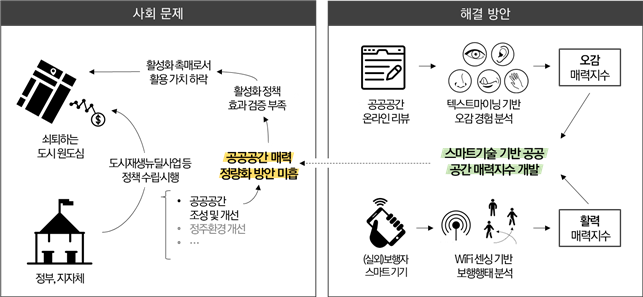
\includegraphics{../image/projectMainImage.png}

\hypertarget{uxbc1cuxd45c-uxd3c9uxac00}{%
\subsubsection{발표 평가}\label{uxbc1cuxd45c-uxd3c9uxac00}}

서류 평가를 통과했다는 메일을 한달 후에 받고 4월 18일 발표 평가를 했다.
평가는 비대면(온라인)으로 제출기한까지 1) 발표자료(15p 이내 PDF), 2)
발표영상(7분이내 발표자료를 설명하는 Zoom 녹화본)을 만들어 보냈다.

발표 당일은 정해진 시간에 Zoom 링크를 통해 평가장에 입장하고 사전에 보낸
7분 발표영상을 심사위원 4\textasciitilde5명과 같이 본 후, 질의응답
시간을 7분 가졌다. 주로 제시한 기술 설명과 한계점을 물어봤다. 어떤
부분이 독창적인지, 제시한 특허와 어떻게 관련되었는지를 대답했다.
해외교육을 신청했기에 미국에서 가능한 사업인지에 대답하고, 영어로
질문하고 답하는 시간도 마지막에 짧게 가졌다.

발표 후, 일주일 내로 최종 선정 메일을 받았다. 아이템에 도움 되는 참고
의견도 같이 보내준다.

\begin{figure}

{\centering 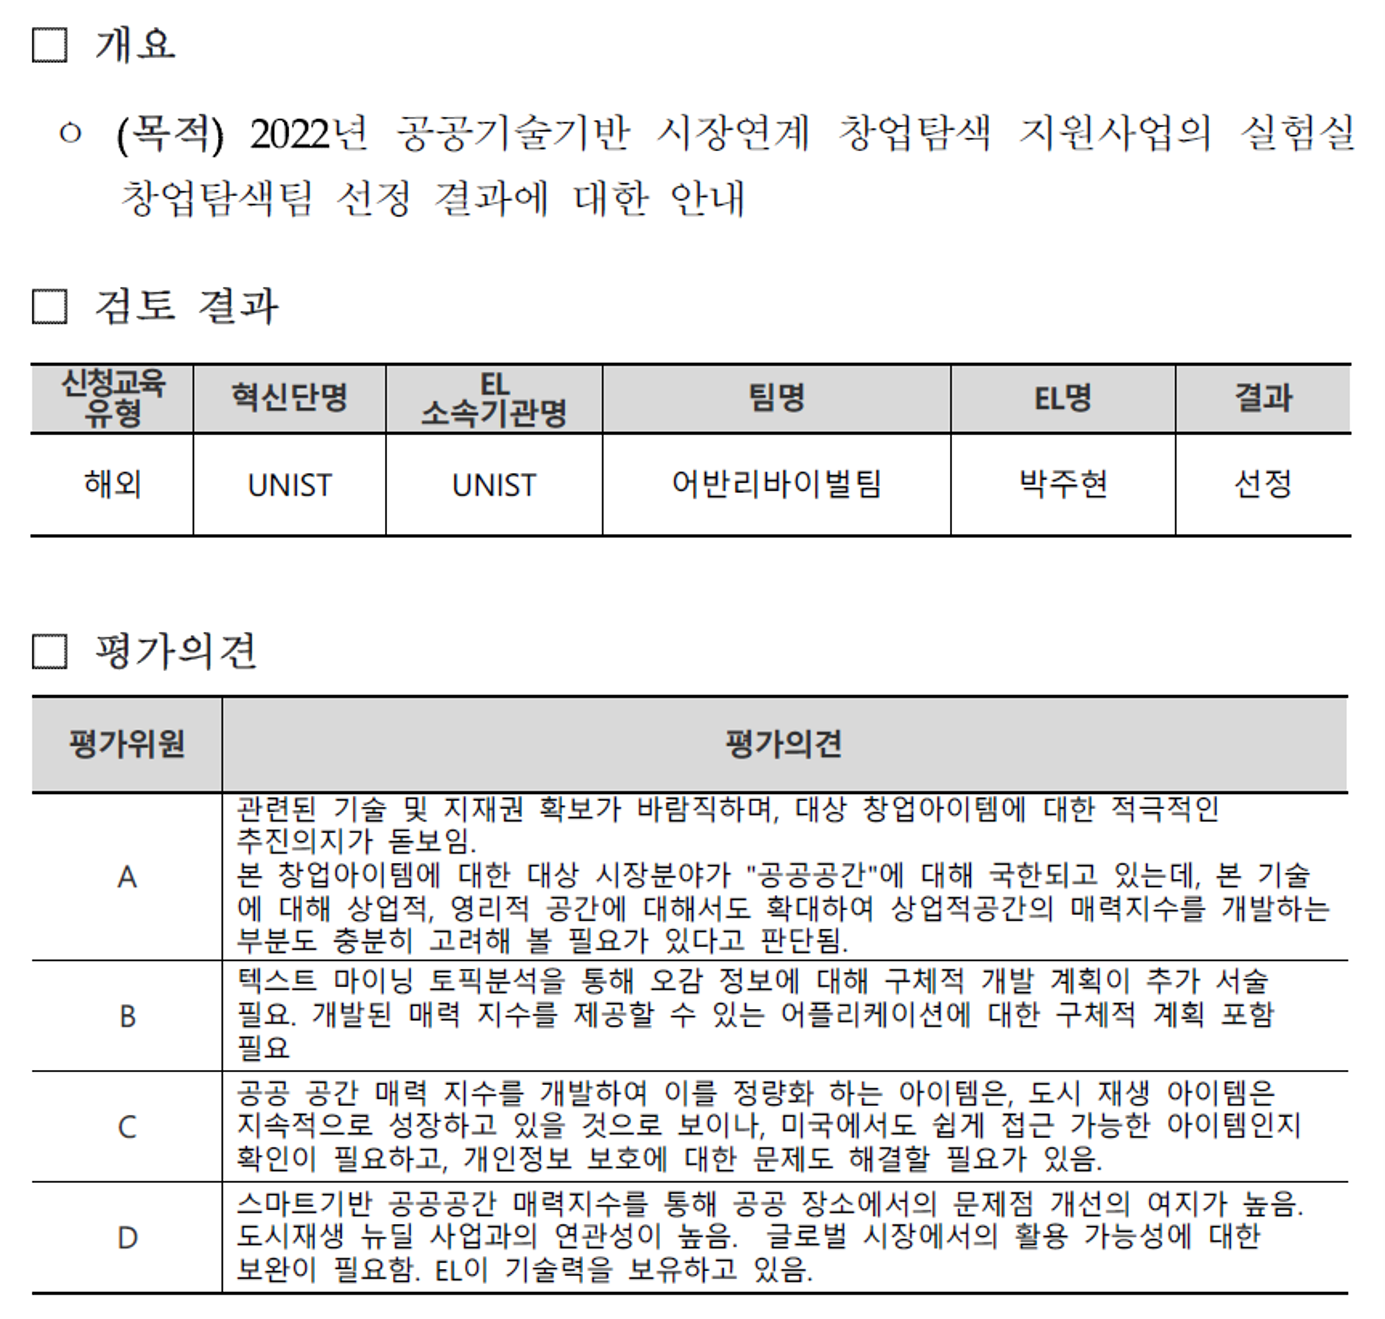
\includegraphics{../image/i-core-opinion.png}

}

\caption{API-intro}

\end{figure}

\begin{center}\rule{0.5\linewidth}{0.5pt}\end{center}

\hypertarget{uxae30uxcd08-uxcc3duxc5c5uxad50uxc721}{%
\subsection{기초 창업교육}\label{uxae30uxcd08-uxcc3duxc5c5uxad50uxc721}}

이론 위주로 고객 탐색하는 방법론에 대해 주로 배운다. 사업 시작을 알리는
부트캠프와 3일간 합숙교육, 기초교육으로 구성된다.

\hypertarget{uxbd80uxd2b8uxcea0uxd504}{%
\subsubsection{부트캠프}\label{uxbd80uxd2b8uxcea0uxd504}}

6월 8일, 선정된 탐색팀이 처음으로 모여 아이코어 프로그램에 대한 소개를
듣고 탐색팀 간 네트워크를 하는 OT 시간을 가졌다.

1부는 전반적인 사업 소개와 혁신단별 인스트럭터 등 사업 관계자 인사,
그리고 이전 기수의 사례 발표가 진행된다. 2부는 각 혁신단별로 모여서 1분
내외로 자신의 아이템을 설명하고 만들어준 명함을 돌리며 서로 알아가는
시간을 가진다. \includegraphics{../image/bootcamp.png}

\hypertarget{uxae30uxcd08uxad50uxc721}{%
\subsubsection{기초교육}\label{uxae30uxcd08uxad50uxc721}}

창업 아이템으로 비즈니스 모델을 만들어보고 이를 검증하는
고객탐색방법론에 대해 배운다. 2박 3일간 합숙교육과 온라인 중간 점검,
최종 발표로 구성되어 있으며, 공식 일정은
\href{../image/basicEducation_syllabus.png}{여기}를 참고하면 된다.

\hypertarget{uxd569uxc219uxad50uxc721-1uxc77cuxcc28}{%
\paragraph{합숙교육
1일차}\label{uxd569uxc219uxad50uxc721-1uxc77cuxcc28}}

6월 25일, 1일차 오전에는 강당에 모여 한국형 아이코어 교육 과정의 개요와
목표에 대해 배운다. 교육 과정은 \textbf{고객 가치}를 무엇보다도
강조한다. - 스타트업 실패 요인이 기술과 자금 부족, 창업 시기 문제가 아닌
고객이 없기 때문 - 검증된 고객 가치를 담은 비즈니스 모델을 찾을 때까지
실패하며 수정과 보완(pivoting)하는 것이 필요 - 이 실패 과정은 빨라야
하며(fail fast), 성공한 비즈니스 모델을 찾은 다음, 마케팅 비용을
투입하고 기업을 설립하여 비즈니스를 확장하는 것이 적절 - 위 과정을
모델화한 것이 \textbf{스티브블랭크의 고객 개발 모델}
(\href{https://brunch.co.kr/@kbhpmp/31}{참고})

다음엔 \textbf{BMC(Business Model Canvas)}, 자신의 스타트업 아이템의
비즈니스 모델을 구체화하는 과정을 돕는 그래픽 템플릿을 배운다. 사업에
필요한 9개 핵심 요소로 구성된 BMC를 만들다보면 내가 어떤 사업을
하려는지를 체계적으로 고민할 수 있다
(\href{https://brunch.co.kr/@givemore/3}{참고}).

\hypertarget{uxae30uxcd08uxad50uxc721-1}{%
\subsubsection{기초교육}\label{uxae30uxcd08uxad50uxc721-1}}

창업 아이템으로 비즈니스 모델을 만들어보고 이를 검증하는
고객탐색방법론에 대해 배운다. 2박 3일 꽉찬 교육으로 공식 일정은
\href{../image/basicEducation_syllabus.png}{여기}를 참고하면 된다.

\hypertarget{uxae30uxcd08uxad50uxc721-1uxc77cuxcc28}{%
\paragraph{기초교육
1일차}\label{uxae30uxcd08uxad50uxc721-1uxc77cuxcc28}}

6월 25일, 1일차 오전에는 강당에 모여 강의를 들었다. 먼저 한국형 아이코어
교육 과정의 개요와 목표를 배웠고 주요 내용은 다음과 같다. - \textbf{고객
가치를 중심으로} 생각하라 - 스타트업 실패 요인은 기술과 자금 부족,
창업시기 문제가 아닌 고객이 없기 때문 - 스타트업은 실패의 연속이며, 고객
가치가 검증된 비즈니스 모델을 찾을 때까지 실패하면서 수정·보완(pivoting)
필요 - 주요 가설을 고객 인터뷰를 통해 검증하고 빠른 실패(fail fast)를
겪는 것이 필요 - 성공가능한 비즈니스 모델을 찾은 다음, 마케팅 비용을
투입하고 기업을 설립하여 비즈니스 확장

위 과정을 모델화한 것이 \textbf{스티브블랭크의 고객 개발 모델}이다. 더
자세한 정보는 \href{https://brunch.co.kr/@kbhpmp/31}{여기}에서 볼 수
있다.

다음 교육에서는 \textbf{BMC(Business Model Canvas)}를 배웠다. - BMC란?
스타트업 아이템의 비즈니스 모델을 구체화하는 과정을 돕는 그래픽 탬플릿 -
사업에 필요한 9개 핵심 요소로 구성된 BMC를 만들다보면 내가 어떤 사업을
하려는지를 체계적으로 고민
(\href{https://brunch.co.kr/@givemore/3}{여기} 참고)
\textgreater\textgreater\textgreater\textgreater\textgreater\textgreater\textgreater{}
Stashed changes

오후에는 혁신단별로 방에 따로 들어가 앉아 자신의 아이템으로 BMC를
작성하고 발표하는 시간을 가졌다. 1시간 동안 BMC를
\href{http://www.bcb.or.kr/}{BCB 웹사이트}에 작성하고 \textbf{과제 1}을
만들어 업로드 한다. 이후 각 팀별로 과제 1을 5분 동안 발표하고 5분
피드백을 듣는다. 저녁을 먹고나서는 인스트럭터와 1:1로 10분간 피드백
시간을 별도로 가진다.

\hypertarget{uxd569uxc219uxad50uxc721-2uxc77cuxcc28}{%
\paragraph{합숙교육
2일차}\label{uxd569uxc219uxad50uxc721-2uxc77cuxcc28}}

2일차는 고객 인터뷰를 수행하는 방법과 모의 인터뷰 실습을 진행한다.
오전에는 고객 인터뷰 필요성과 설계, 수행 방법에 대해 배운다. 인터뷰가
귀찮은 과정은 맞지만 하지 않았을 때 겪는 어려움은 이 두 클립을 보면 알
수 있다 \href{https://www.youtube.com/watch?v=uPhHPO98M84\&t=236s}{(1,}
\href{https://www.youtube.com/watch?v=mrR3CdaPCBY}{2)}.

오후에는 배운 인터뷰 내용을 실습하는 시간을 가진다. 점심 이후 1시간 동안
인터뷰 수행을 위한 비즈니스 가설 및 인터뷰 전략을 구상한다. 이후 3시간
동안 혁신단 다른 팀과 다른 혁신단 팀들과 모의 인터뷰를 진행한다.
\includegraphics{../image/basicEducation_interview_1.png} 총 10팀의 모의
인터뷰 수행건을 정리한 \textbf{과제 2}는 2일차 밤까지 업로드한다.
1일차와 마찬가지로 저녁 이후 인스트럭터와 피드백 시간을 가지며 인터뷰
수행한 것에 대한 조언을 듣는다.

\hypertarget{uxd569uxc219uxad50uxc721-3uxc77cuxcc28}{%
\paragraph{합숙교육
3일차}\label{uxd569uxc219uxad50uxc721-3uxc77cuxcc28}}

3일차는 교육 없이 합숙교육으로 배운 내용을 오전에 발표했다. BMC로 사업
컨셉을 설명하고, 모의 인터뷰로 검증하고자 하는 것을 가치제안모델과
비즈니스모델 가설 페이지로 전달했다. 이후 각 인터뷰를 정리한
고객인터뷰기록과 최종 인사이트 도출 페이지로 모의 인터뷰 수행 결과를
발표했다.

\begin{figure}

{\centering 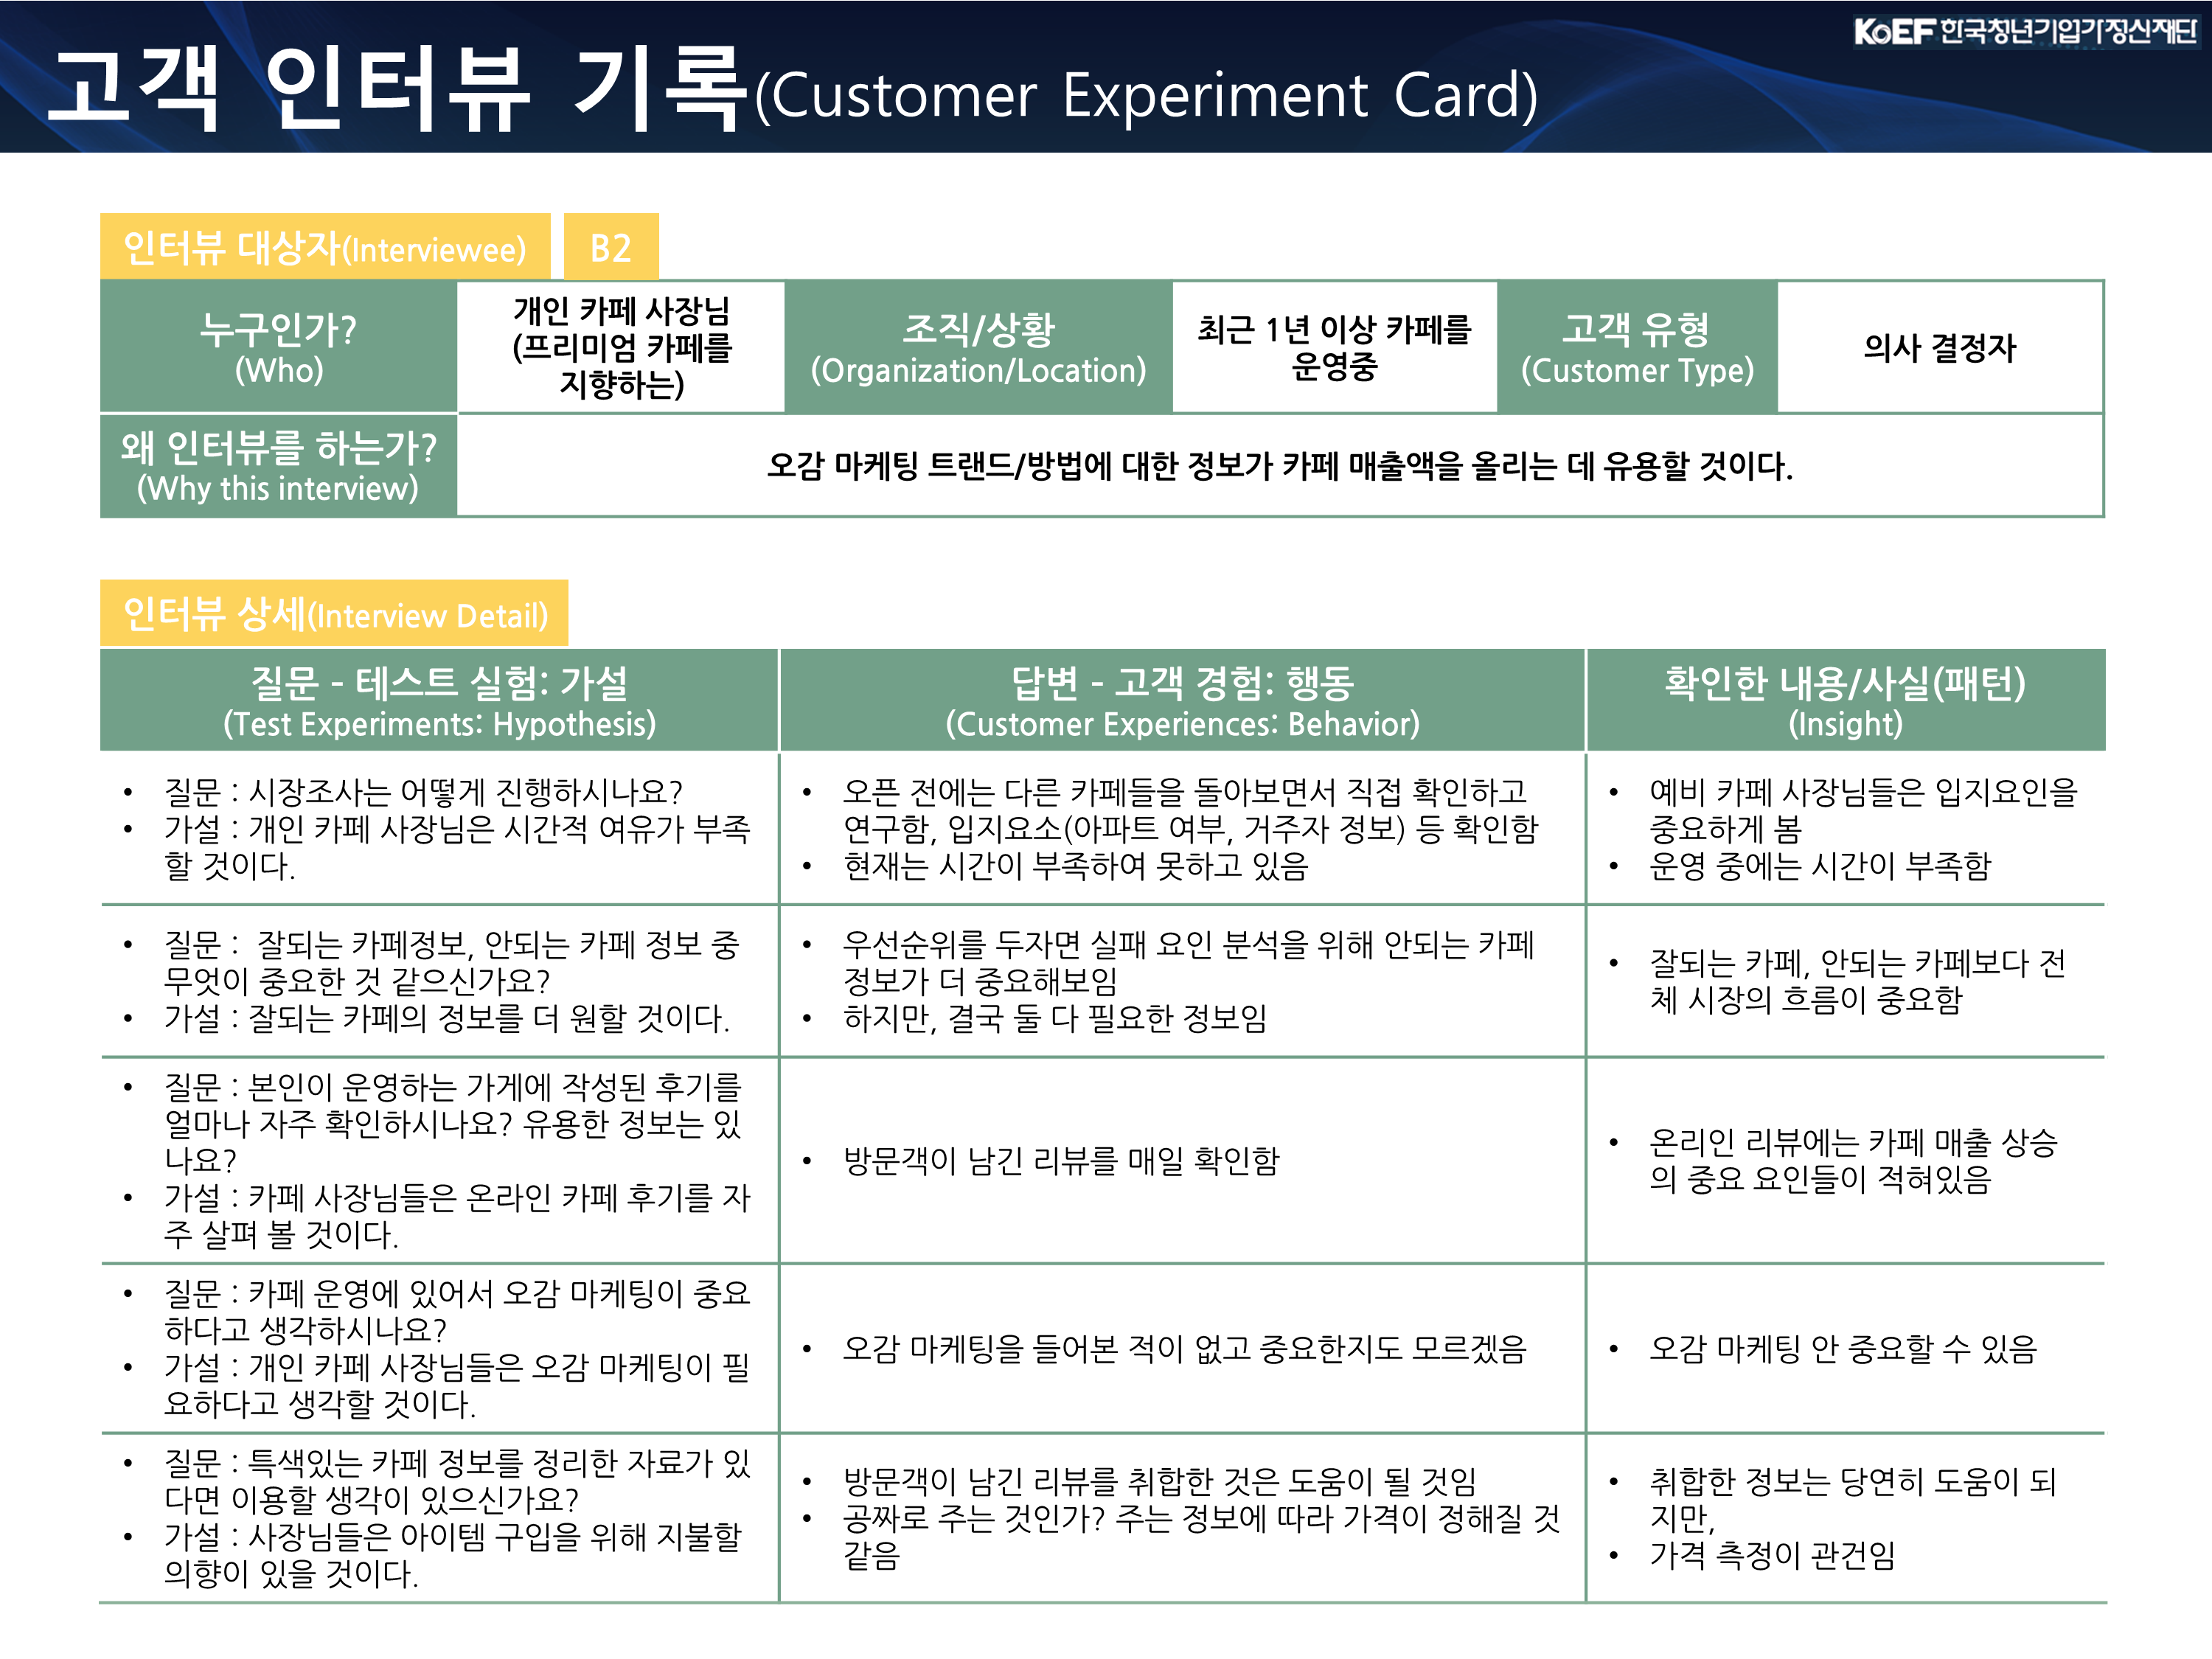
\includegraphics{../image/basicEducation_assignment2.png}

}

\caption{여기}

\end{figure}

\hypertarget{uxcd5cuxc885uxbc1cuxd45c}{%
\paragraph{최종발표}\label{uxcd5cuxc885uxbc1cuxd45c}}

합숙 교육이 끝나고 최종발표까지 2주간 실제 고객 인터뷰 15건을 수행한다.
\includegraphics{../image/basicEducation_interview_real.png}

이 인터뷰를 정리한 \textbf{과제 3}으로 10분 발표와 5분 피드백 시간을
가진다. 앞서 말한대로 인터뷰로 검증되지 않은 비즈니스 모델인 경우 수정
및 보완 하는 것이 당연하므로, 이 과제 3도 이 과정이 포함된다.
\includegraphics{../image/basicEducation_assignment3.png}
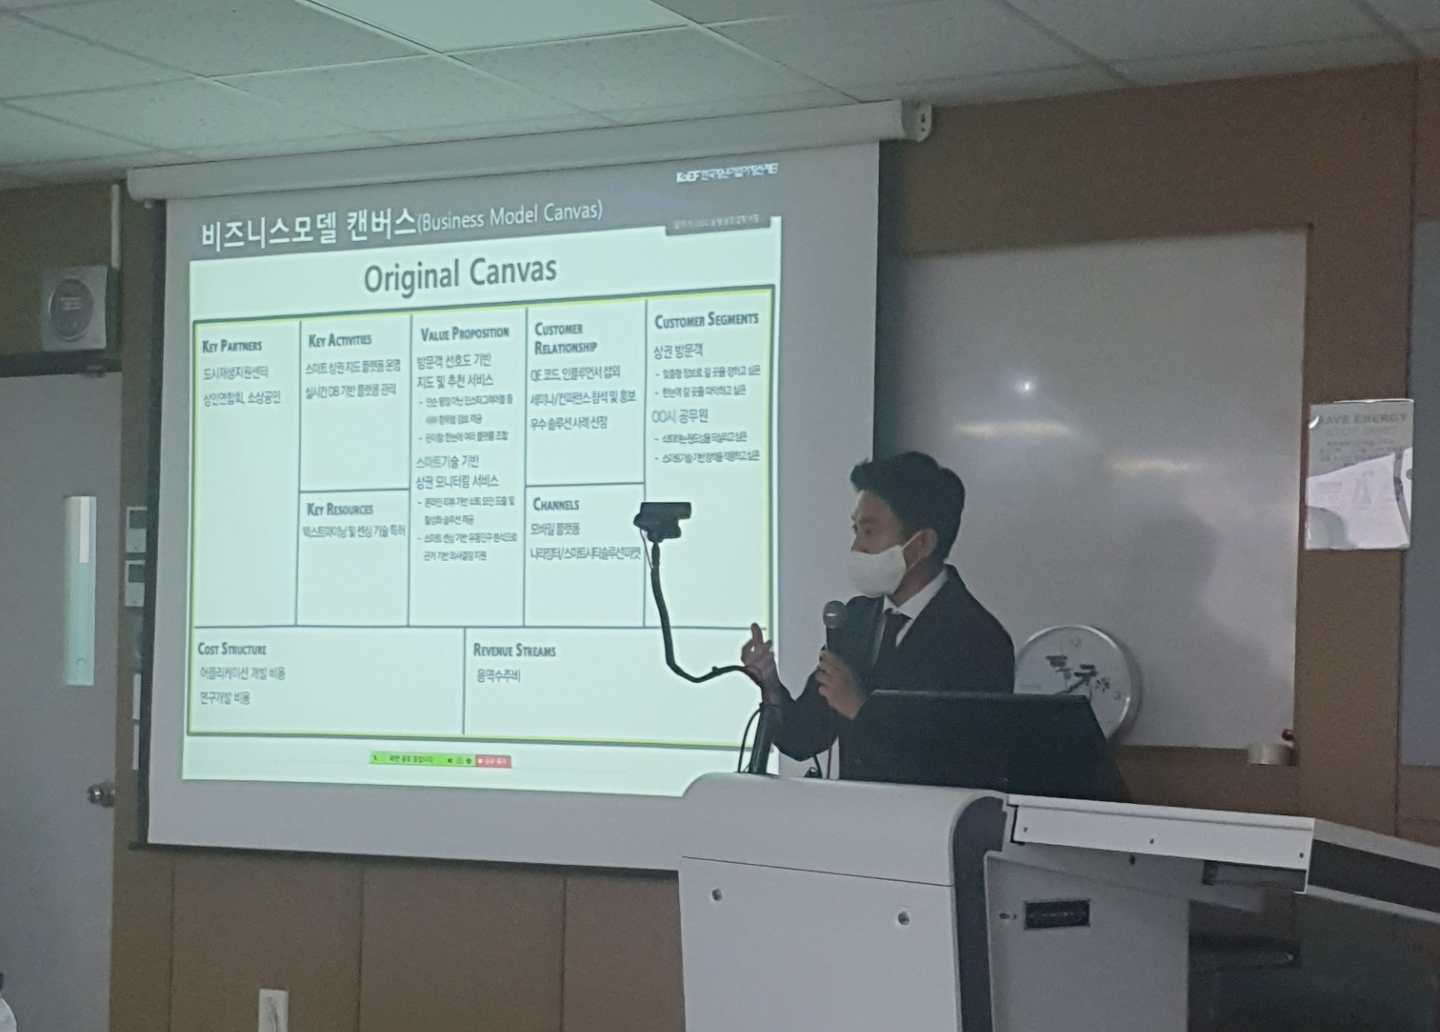
\includegraphics{../image/basicEducation_assignment3_present.png}

피봇 과정을 거친다면 BMC도 바뀌게 된다. 처음 BMC와 바뀐 BMC도 발표하며,
얼마나 바뀐 지를 인스트럭터 평가자가 눈여겨 본다.
\includegraphics{../image/basicEducation_BMC_revised.png}

\hypertarget{uxae30uxcd08uxad50uxc721-uxc18cuxacb0}{%
\paragraph{기초교육 소결}\label{uxae30uxcd08uxad50uxc721-uxc18cuxacb0}}

\hypertarget{uxc900uxbe44uxd55c-uxc544uxc774uxd15cuxc73cuxb85c-uxae30uxcd08uxad50uxc721uxc740-uxb05duxae4cuxc9c0-uxc218uxd589uxd558uxace0-uxcd5cuxc885-uxbc1cuxd45cuxc5d0uxc11c-uxc218uxc815uxd558uxc790}{%
\subparagraph{1. 준비한 아이템으로 기초교육은 끝까지 수행하고 최종
발표에서
수정하자}\label{uxc900uxbe44uxd55c-uxc544uxc774uxd15cuxc73cuxb85c-uxae30uxcd08uxad50uxc721uxc740-uxb05duxae4cuxc9c0-uxc218uxd589uxd558uxace0-uxcd5cuxc885-uxbc1cuxd45cuxc5d0uxc11c-uxc218uxc815uxd558uxc790}}

우리 팀은 기초교육 첫 단추를 잘못 끼워 교육 내내 고생했다. 과제 1
발표부터 우리는 제출한 아이템의 고객인 공공공간 관리자, 공무원이 아닌
소상공인으로 첫페이지부터 소개를 했었다. 교육(인터뷰)를 수행하지도 않고
아이템을 바꾸는 경우는 지원서 합격을 위해 그럴싸한 아이템으로 지원하고
바꾸는 경우로 의심받을 수 있다고 한다. 인터뷰 이후 수정 및 보완은 아주
당연한 과정이므로, 처음 제출한 아이템이 이상하더라도 계속해서 교육을
수행하고 마지막에 바꾸기를 추천한다.

\hypertarget{uxc900uxbe44uxd55c-uxc544uxc774uxd15cuxc73cuxb85c-bmc-uxbbf8uxb9ac-uxb9ccuxb4e4uxc5b4uxc624uxc790}{%
\subparagraph{2. 준비한 아이템으로 BMC 미리
만들어오자}\label{uxc900uxbe44uxd55c-uxc544uxc774uxd15cuxc73cuxb85c-bmc-uxbbf8uxb9ac-uxb9ccuxb4e4uxc5b4uxc624uxc790}}

1시간만에 BMC를 완성하기가 정말 쉽지 않아서 미리 생각해오는게 필요하다.
아래는 만든 첫번째 BMC인데 잘못된 점이 아주 많지만 기록으로 여기
올려둔다. 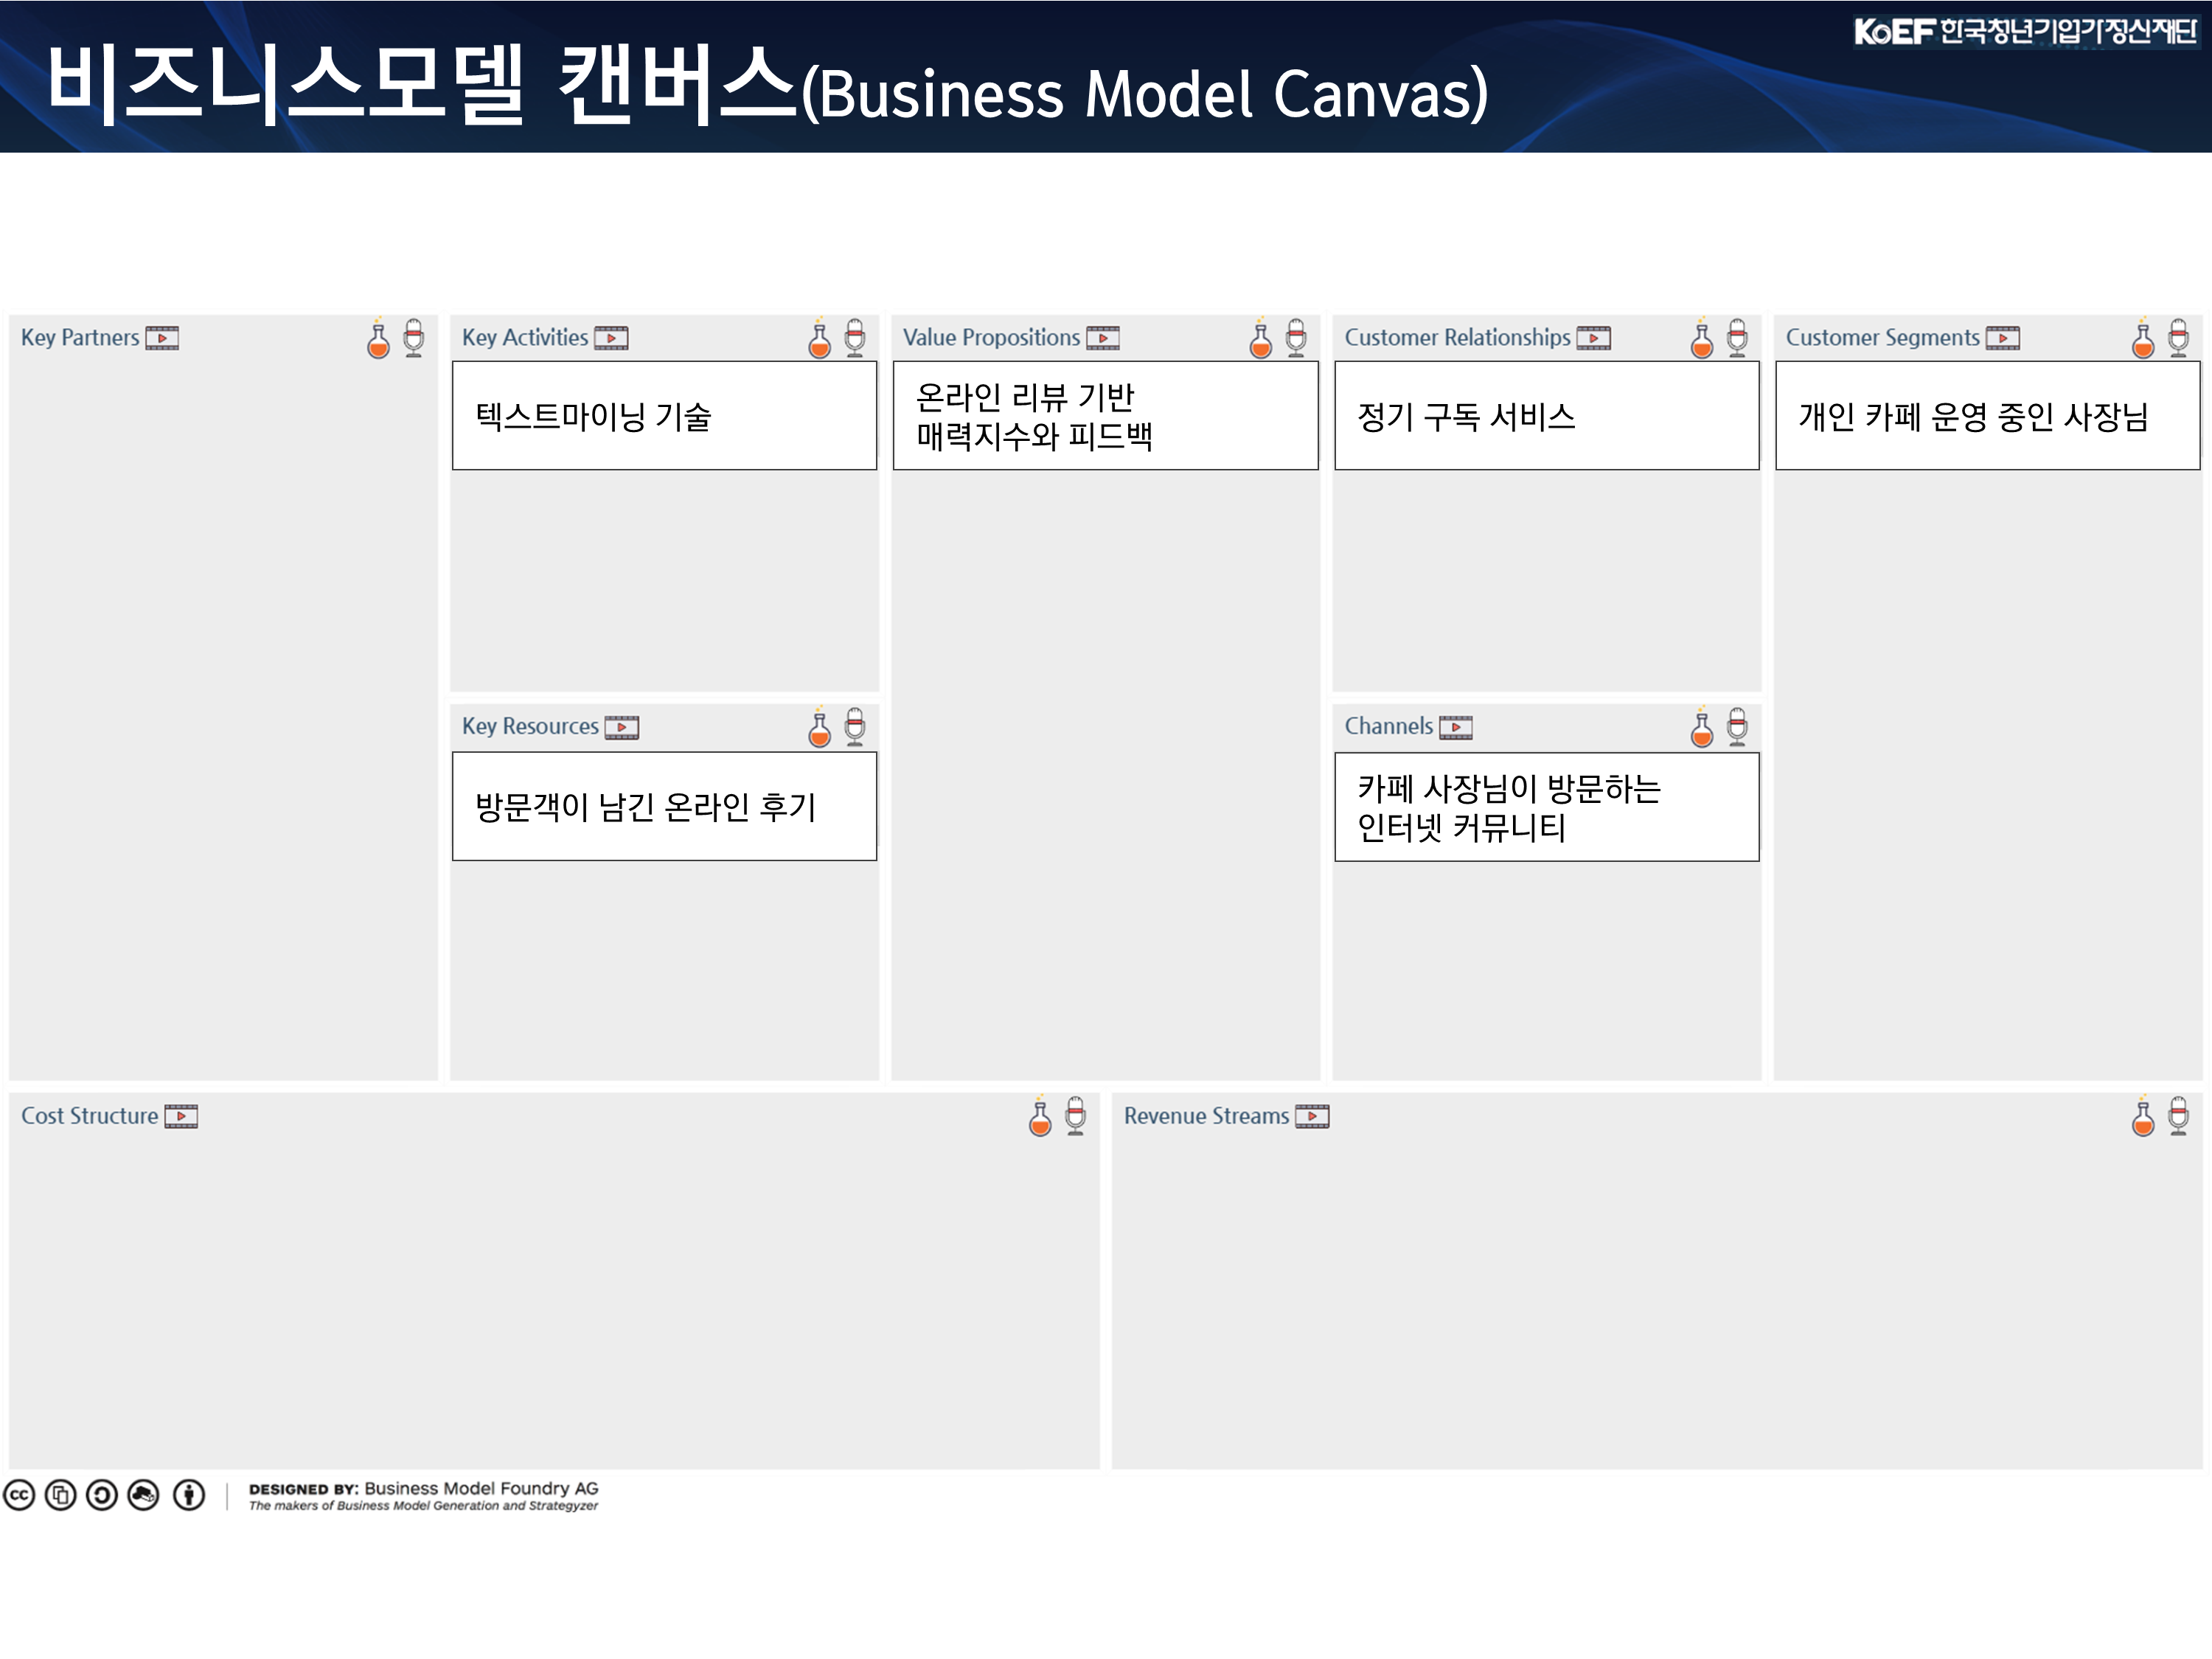
\includegraphics{../image/basicEducation_BMC_1.png}

\hypertarget{uxbaa8uxc758-uxc778uxd130uxbdf0uxb294-uxc0c1uxb300uxc5d0uxac8c-uxad6cuxccb4uxc801uxc778-uxd398uxb974uxc18cuxb098uxb97c-uxbd80uxc5ecuxd558uxc790}{%
\subparagraph{3. 모의 인터뷰는 상대에게 구체적인 페르소나를
부여하자}\label{uxbaa8uxc758-uxc778uxd130uxbdf0uxb294-uxc0c1uxb300uxc5d0uxac8c-uxad6cuxccb4uxc801uxc778-uxd398uxb974uxc18cuxb098uxb97c-uxbd80uxc5ecuxd558uxc790}}

모의 인터뷰를 하면서 느낀건 인터뷰 상대는 우리와 같은 스타트업 창업자지
진정한 고객이 아니므로, 페르소나를 구체적으로 부여해야 한든 것이다.
고객을 구체적으로 설정하면 좋은 것과 같지, 모의 인터뷰 이전 상대 팀에게
우리 아이템에 대해 밝히지 않으면서 되었으면 하는 고객에 대해 최대한
구체적으로 말하는게 좋았다. 우리는 처음에는 일반적인 소상공인에서,
인터뷰를 수행하면서 카페 사장님, 개인 카페 사장님, 프리미엄 카페
운영하는 사장님으로 좁혀나갔고 더 유의미한 결과를 얻었다.

\hypertarget{uxc2e4uxc804uxad50uxc721}{%
\subsection{실전교육}\label{uxc2e4uxc804uxad50uxc721}}

실전 교육은 국내형과 해외형으로 나눠진다. 우리 팀은 해외형 실전교육을
수행했고 미국 서부로 가 3주간 교육을 받았다. 각 1주를 Core week으로
부르고 수요일마다 모여서 프로그램 경과를 발표한다. 마지막 날은 Demo
day로 최종 발표를 하고 교육은 마무리 된다. 교육 과정은
\href{../file/KIC_UC_Berkeley_Syllabus_2022.docx}{여기}에서 볼 수 있다.

\hypertarget{uxc2e4uxc804uxad50uxc721-1uxc8fcuxcc28}{%
\subsubsection{실전교육
1주차}\label{uxc2e4uxc804uxad50uxc721-1uxc8fcuxcc28}}

미국 도착 다음날 Core week 1 발표가 바로 있다. 프로그램을 등록하고
소개를 간략히 받은 다음, 팀별로 발표가 시작되고 팀 소개를 먼저 한다.
우리는 음식점 온라인 리뷰를 분석해서 고객 경험을 이해하고 다중 평가 기준
점수를 제공해서 1) 방문객에게는 맛집 추천을 2) 소상공인 음식점
주인에게는 컨설팅 서비스를 제공하려고 했다.
\includegraphics{../image/practical_LL1_1.png} 이후 인터뷰 수행 결과와
계획에 대해서 발표한다. 미국에서 인터뷰 기회가 현실적으로 없지만 인터뷰
결과를 발표해야 하므로, 최종 발표 이후 국내 인터뷰를 꾸준히 더 수행해야
한다. 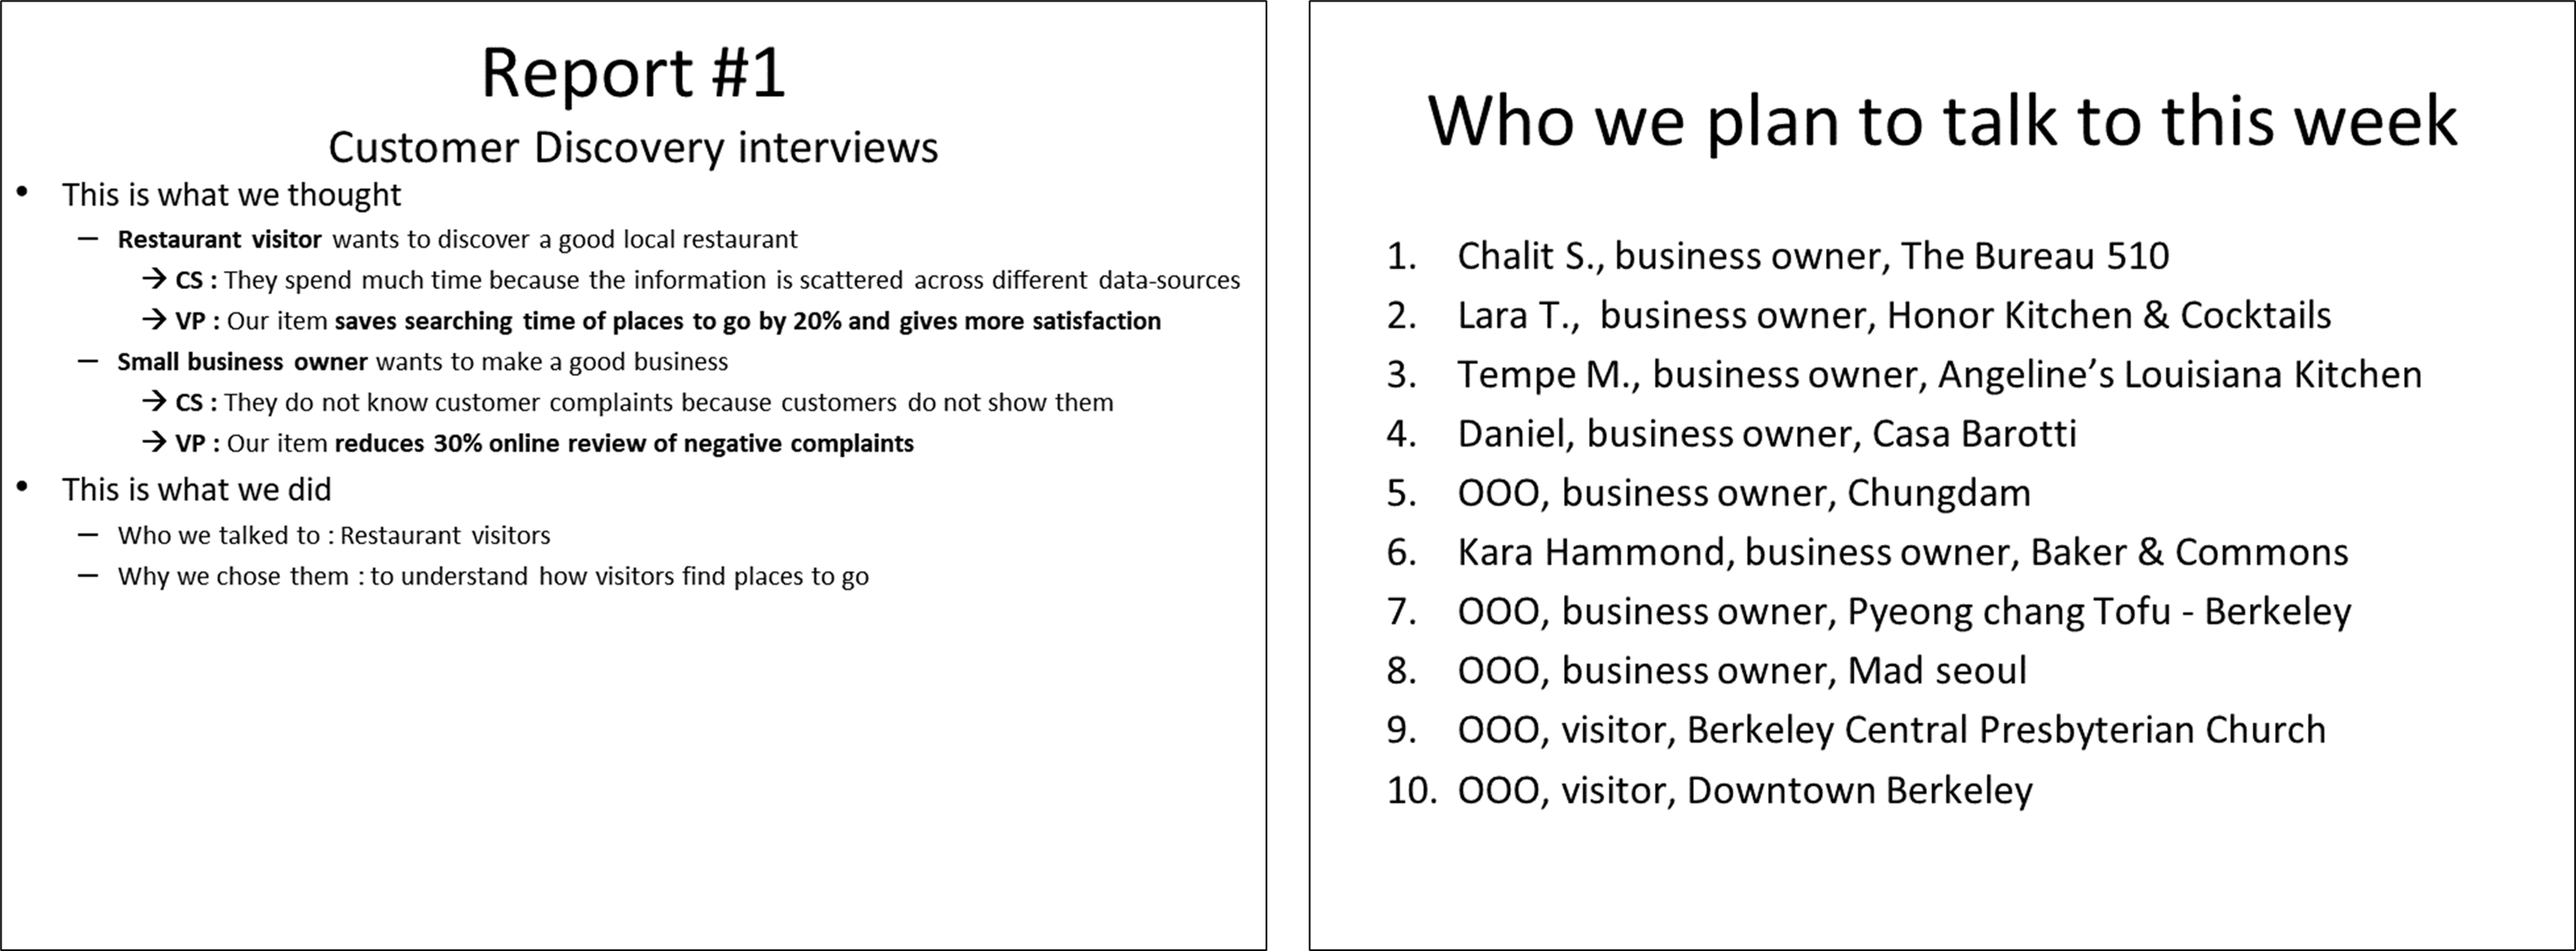
\includegraphics{../image/practical_LL1_2.png} \#\#\# 실전교육
2주차 1주차 수요일부터 일주일간 인터뷰 수행 결과를 2주차 수요일에
발표한다. 첫 부분은 팀 소개와 BMC이고 수정된 것을 발표해도 괜찮다. 우리
팀은 의사결정에 도움을 주는 시스템(decision support system)으로 이름을
바꾸고, 30건이 추가되어 총 35건 인터뷰를 수행했으며 BMC에서는 1)
방문객들에게 맛집 검색 시간을 1/5로 줄여줄 것을, 2) 소상공인에게는
온라인 리뷰 기반 리포트를 제공할 것을 구분지어 발표했다.
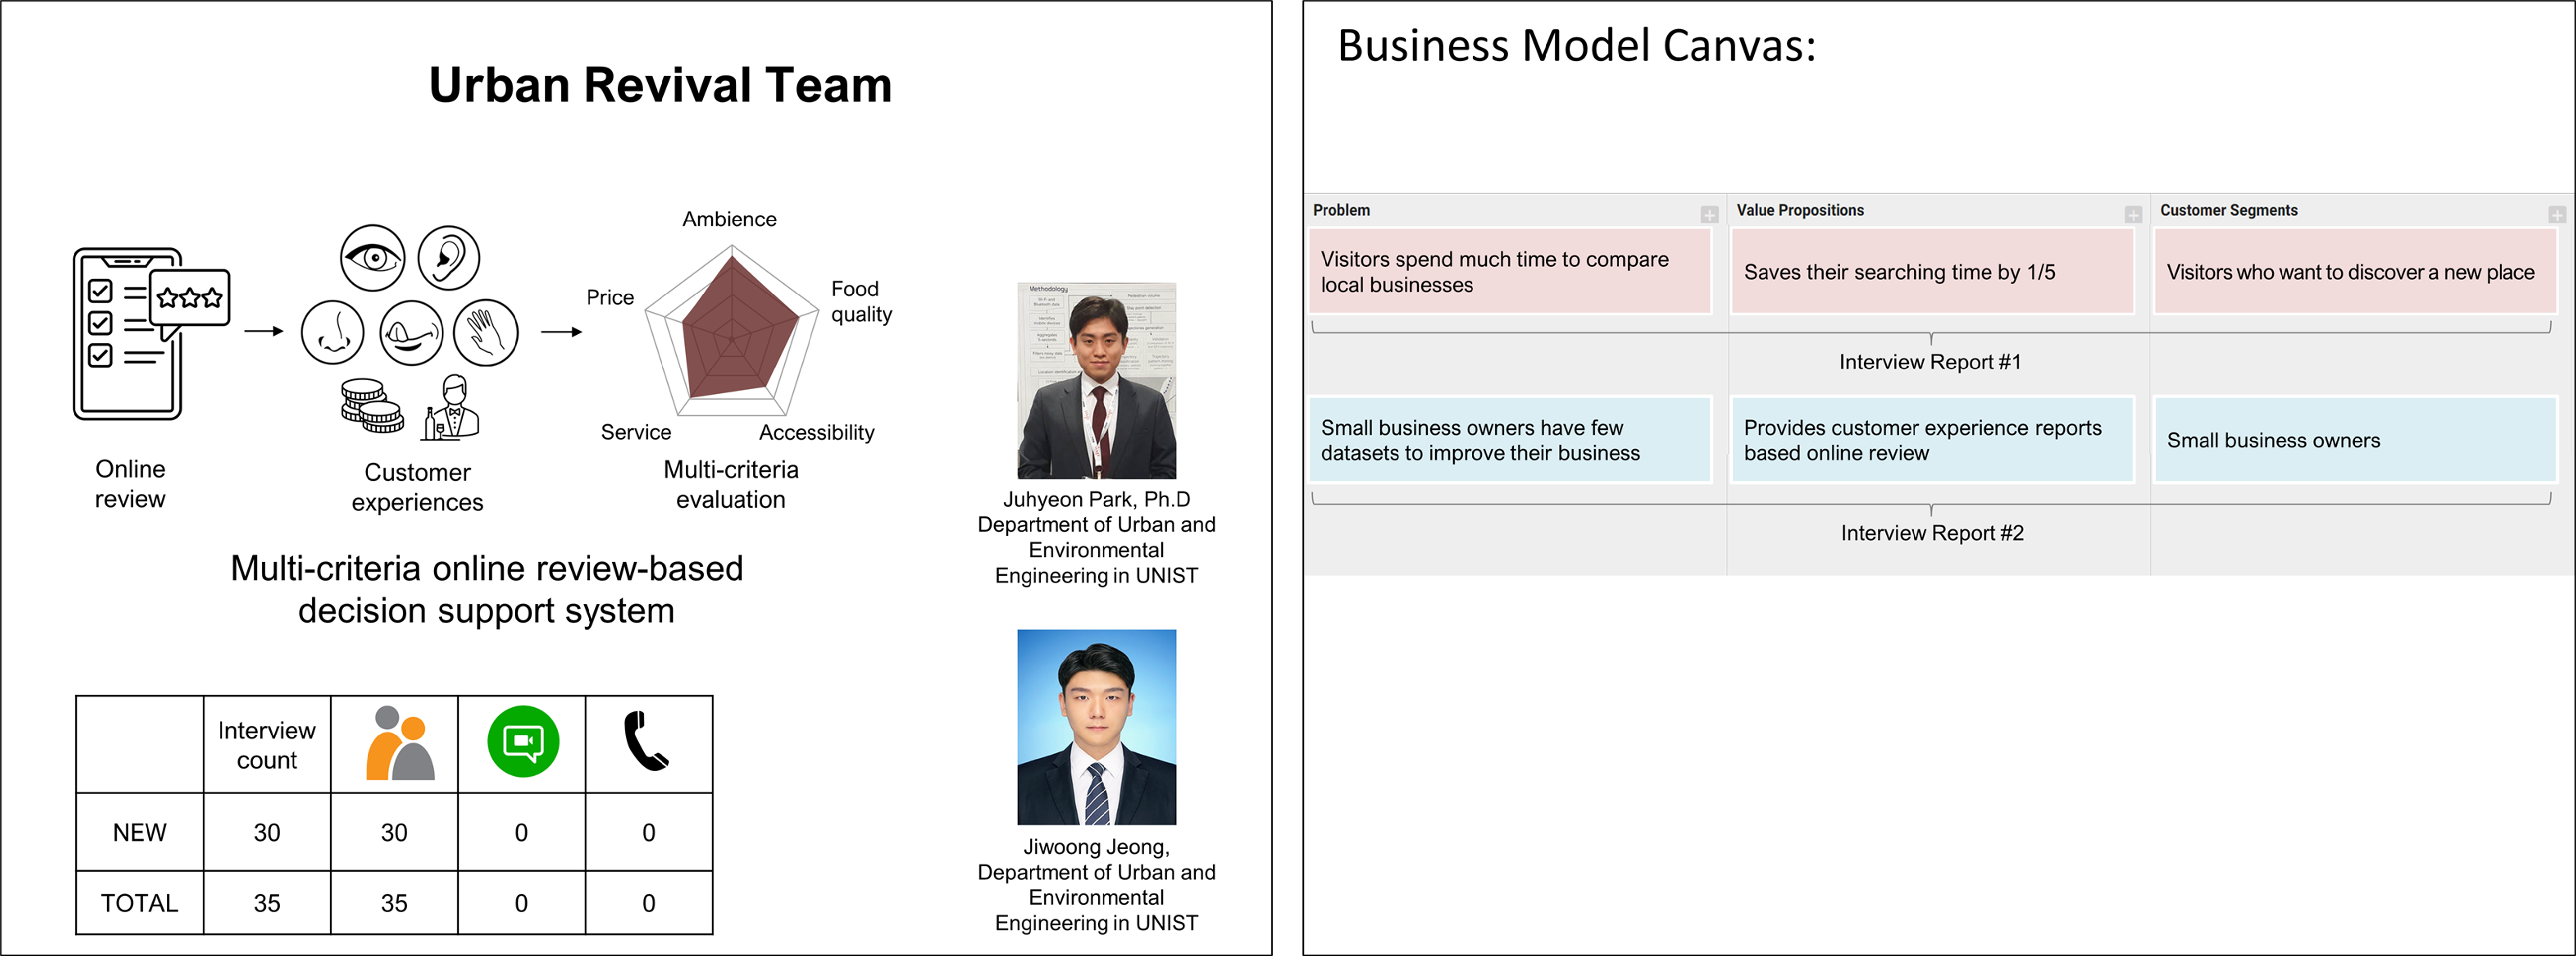
\includegraphics{../image/practical_LL2_1.png} 이후 인터뷰 수행 리포트는
우리가 생각했던 것(\emph{가설})과 수행 했던 것(\emph{실험}), 배운
것(\emph{결과}), 향후 계획(\emph{토론})을 담아 만든다. 인터뷰를 수행하기
전 이 부분에 채워야할 것을 생각하고 설계한다면 더 도움이 될 것 같다.
\includegraphics{../image/practical_LL2_2.png} 발표 마지막엔 BMC를
보여준다. 업데이트된 고객과 고객 문제, 가치 제안을 포함해서 1주차에서
배운 Channels과 Revenue Streams을 추가한다.
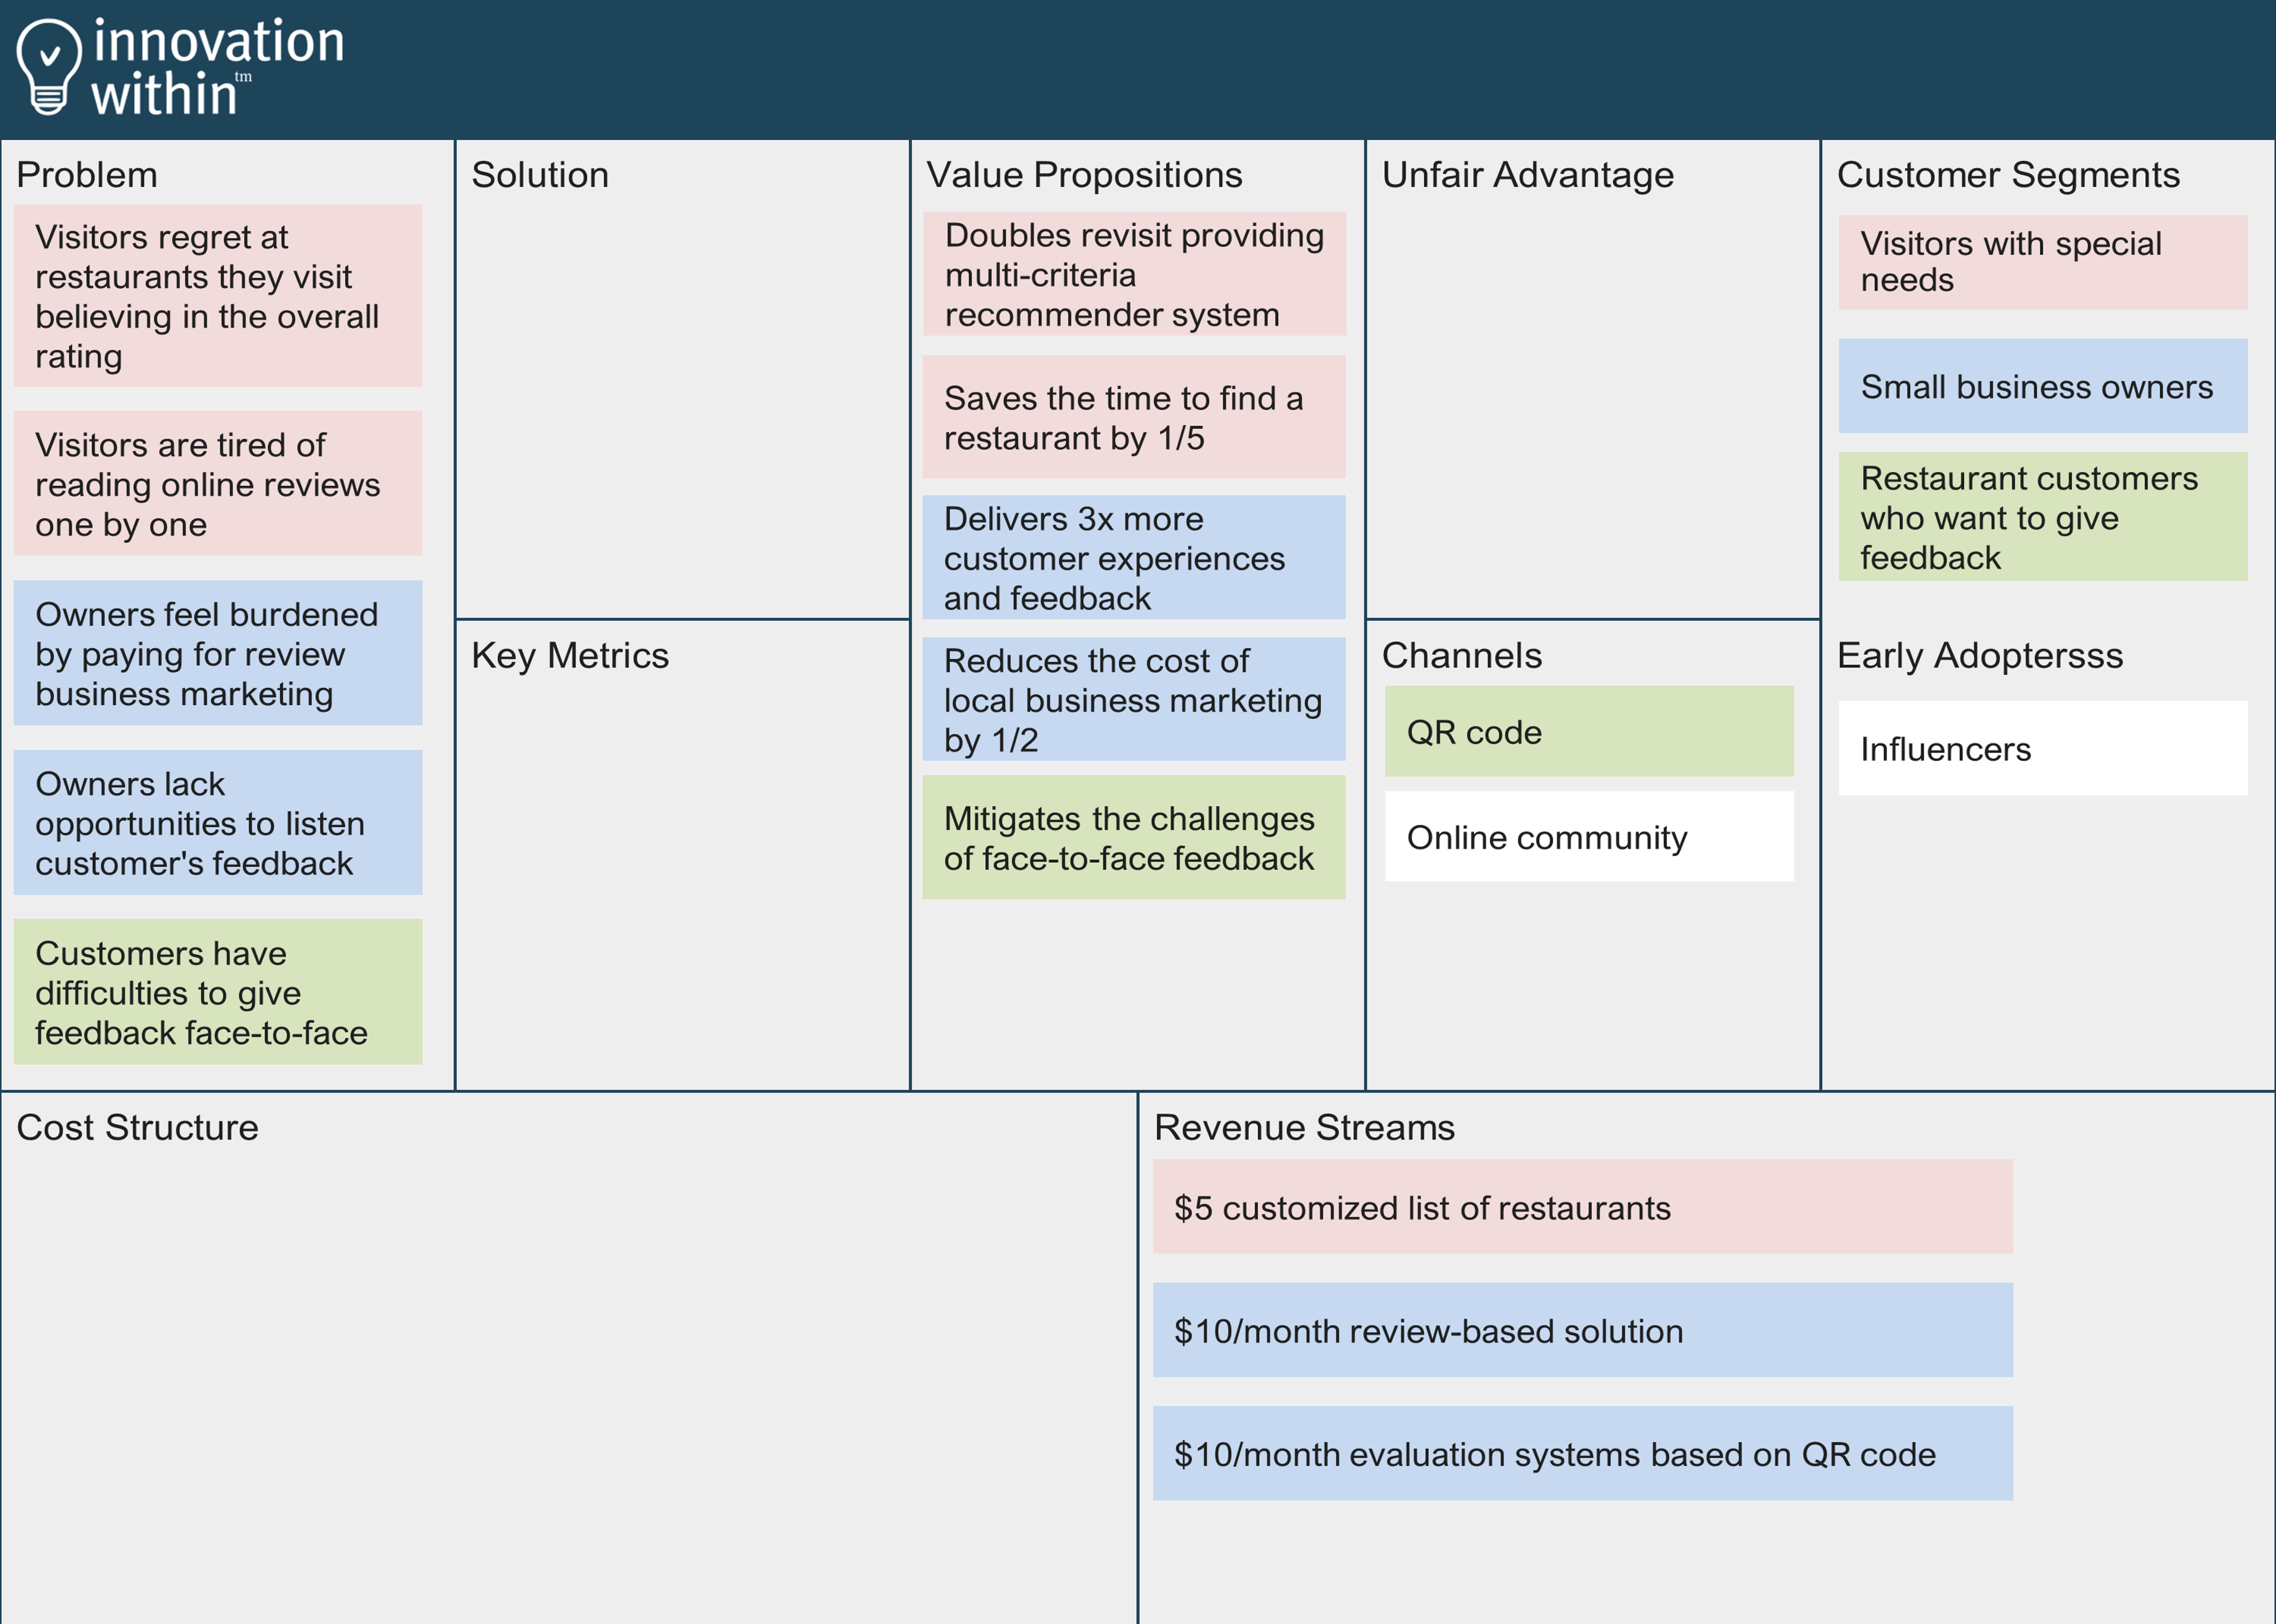
\includegraphics{../image/practical_LL2_3.png}

\hypertarget{uxc2e4uxc804uxad50uxc721-3uxc8fcuxcc28}{%
\subsubsection{실전교육
3주차}\label{uxc2e4uxc804uxad50uxc721-3uxc8fcuxcc28}}

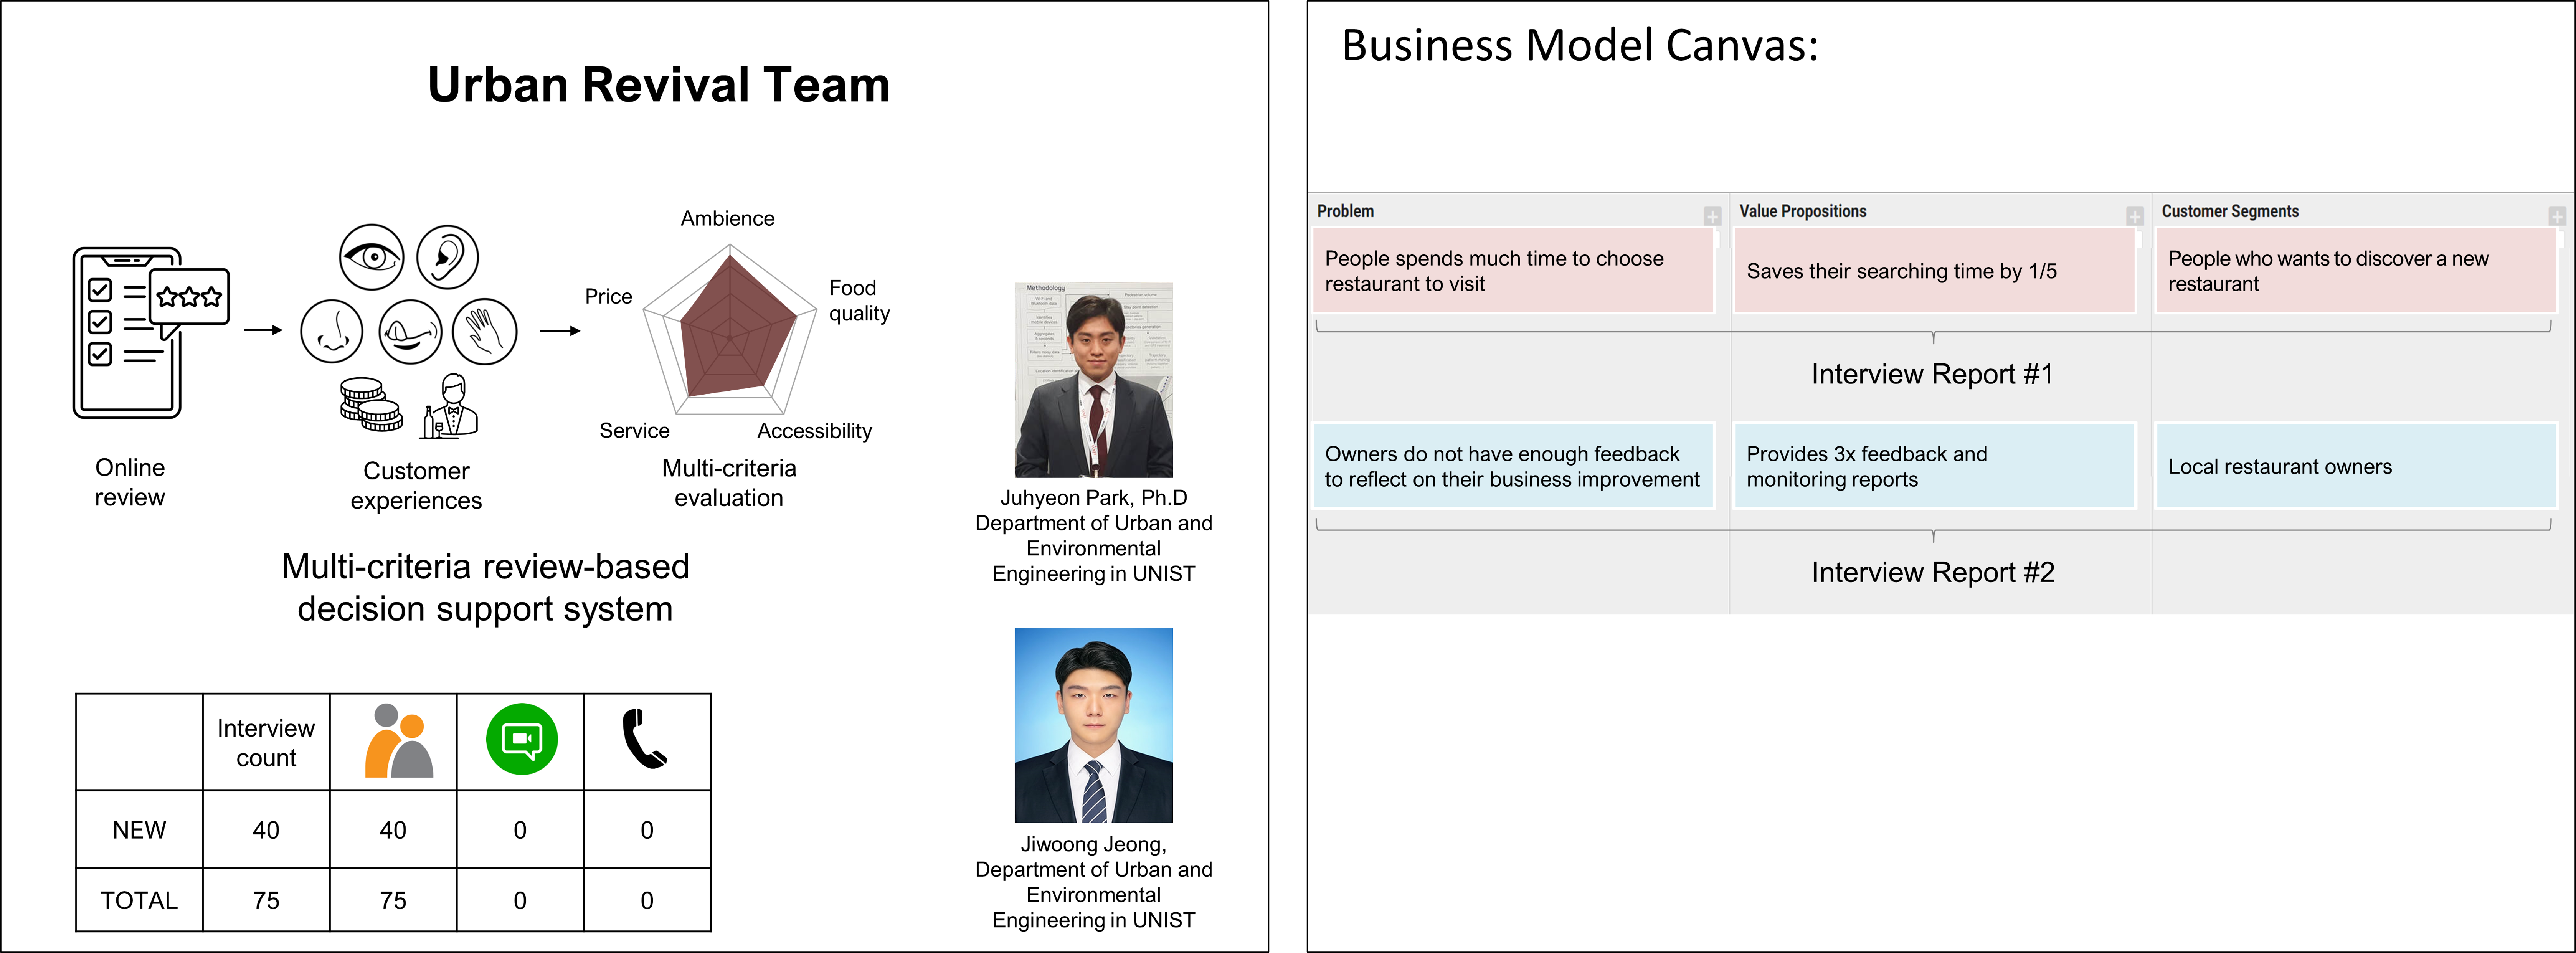
\includegraphics{../image/practical_LL3_1.png}

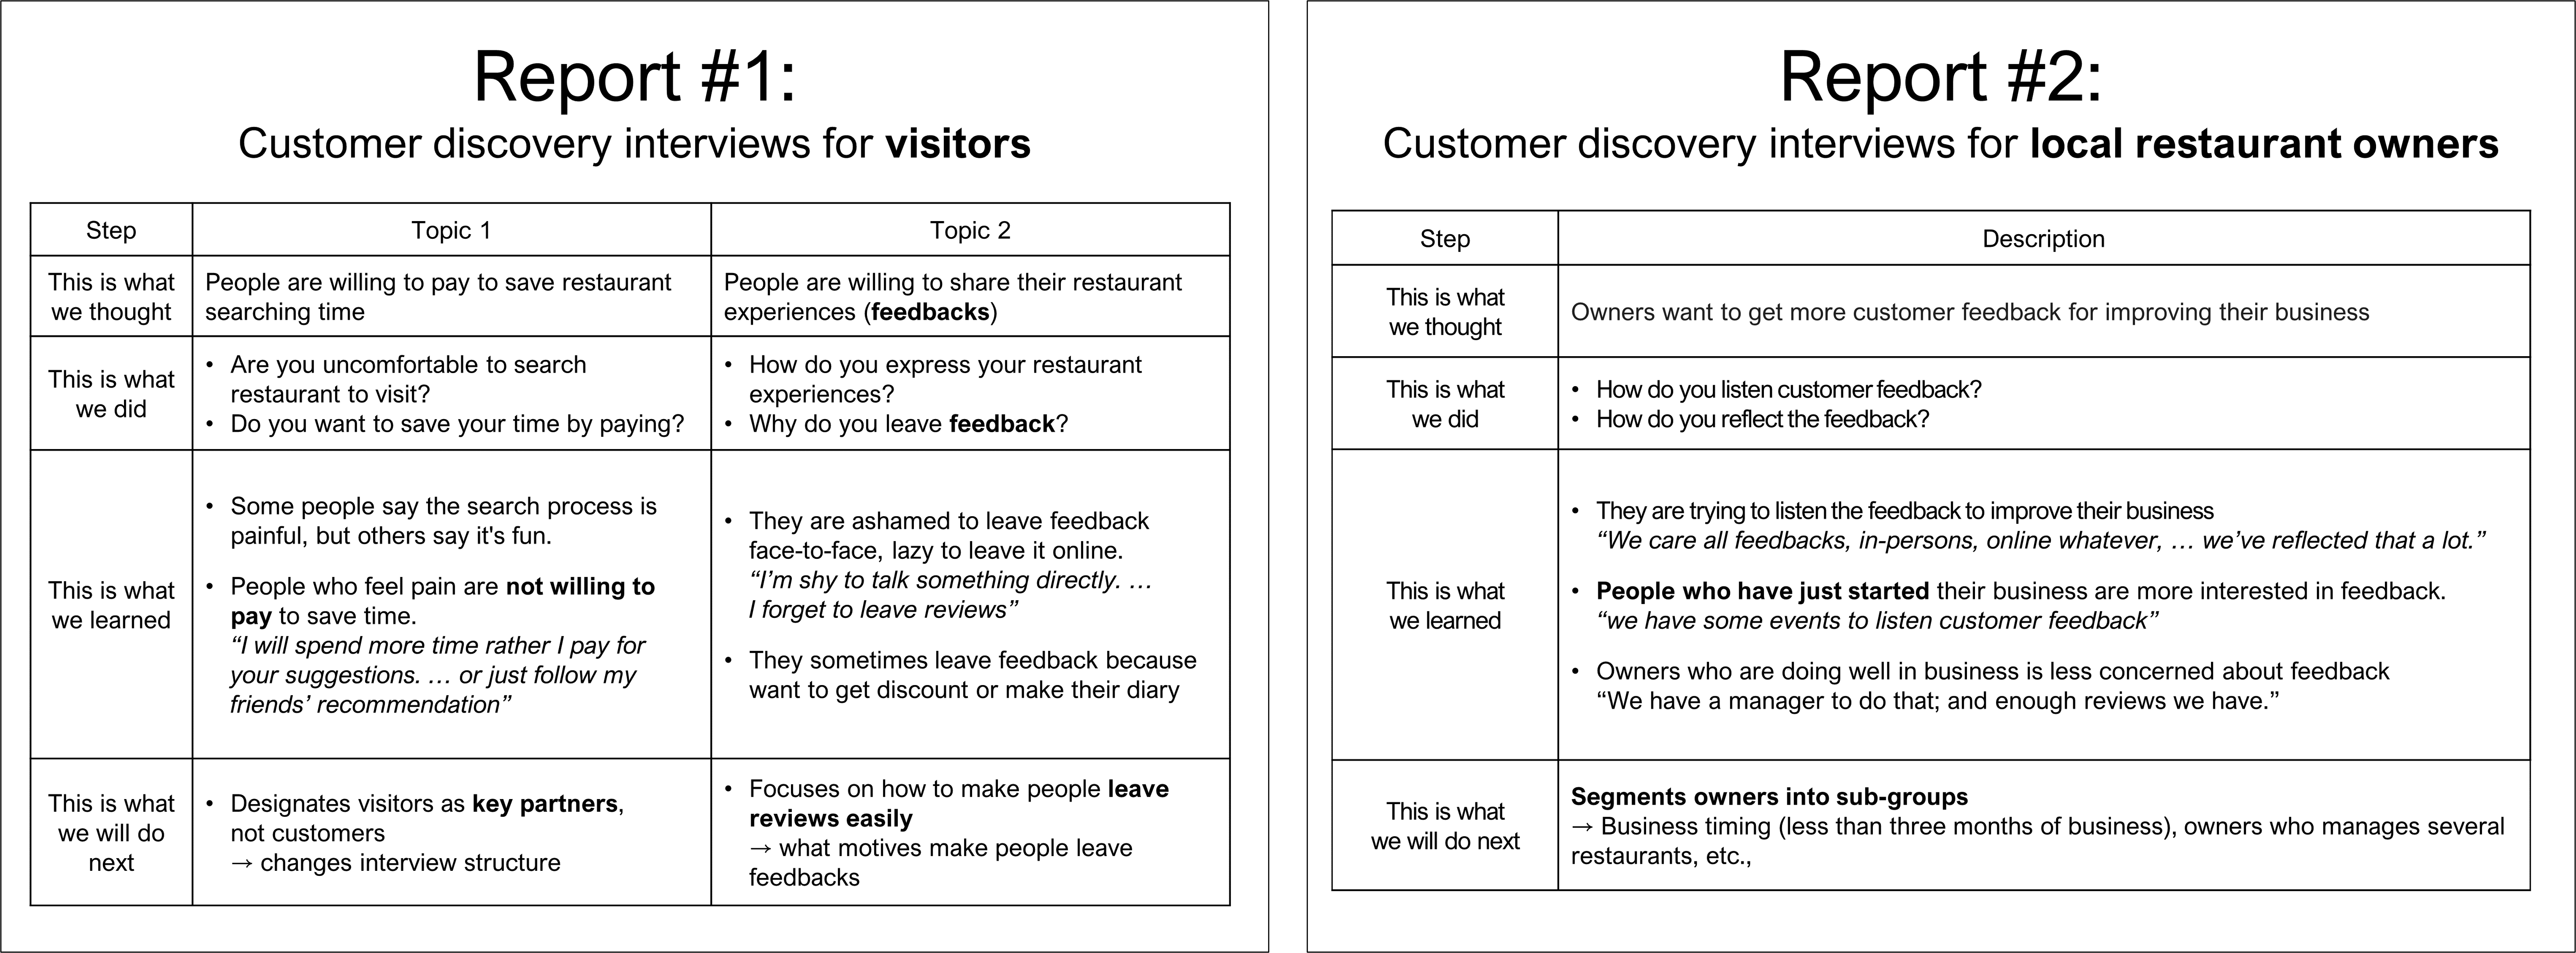
\includegraphics{../image/practical_LL3_2.png}

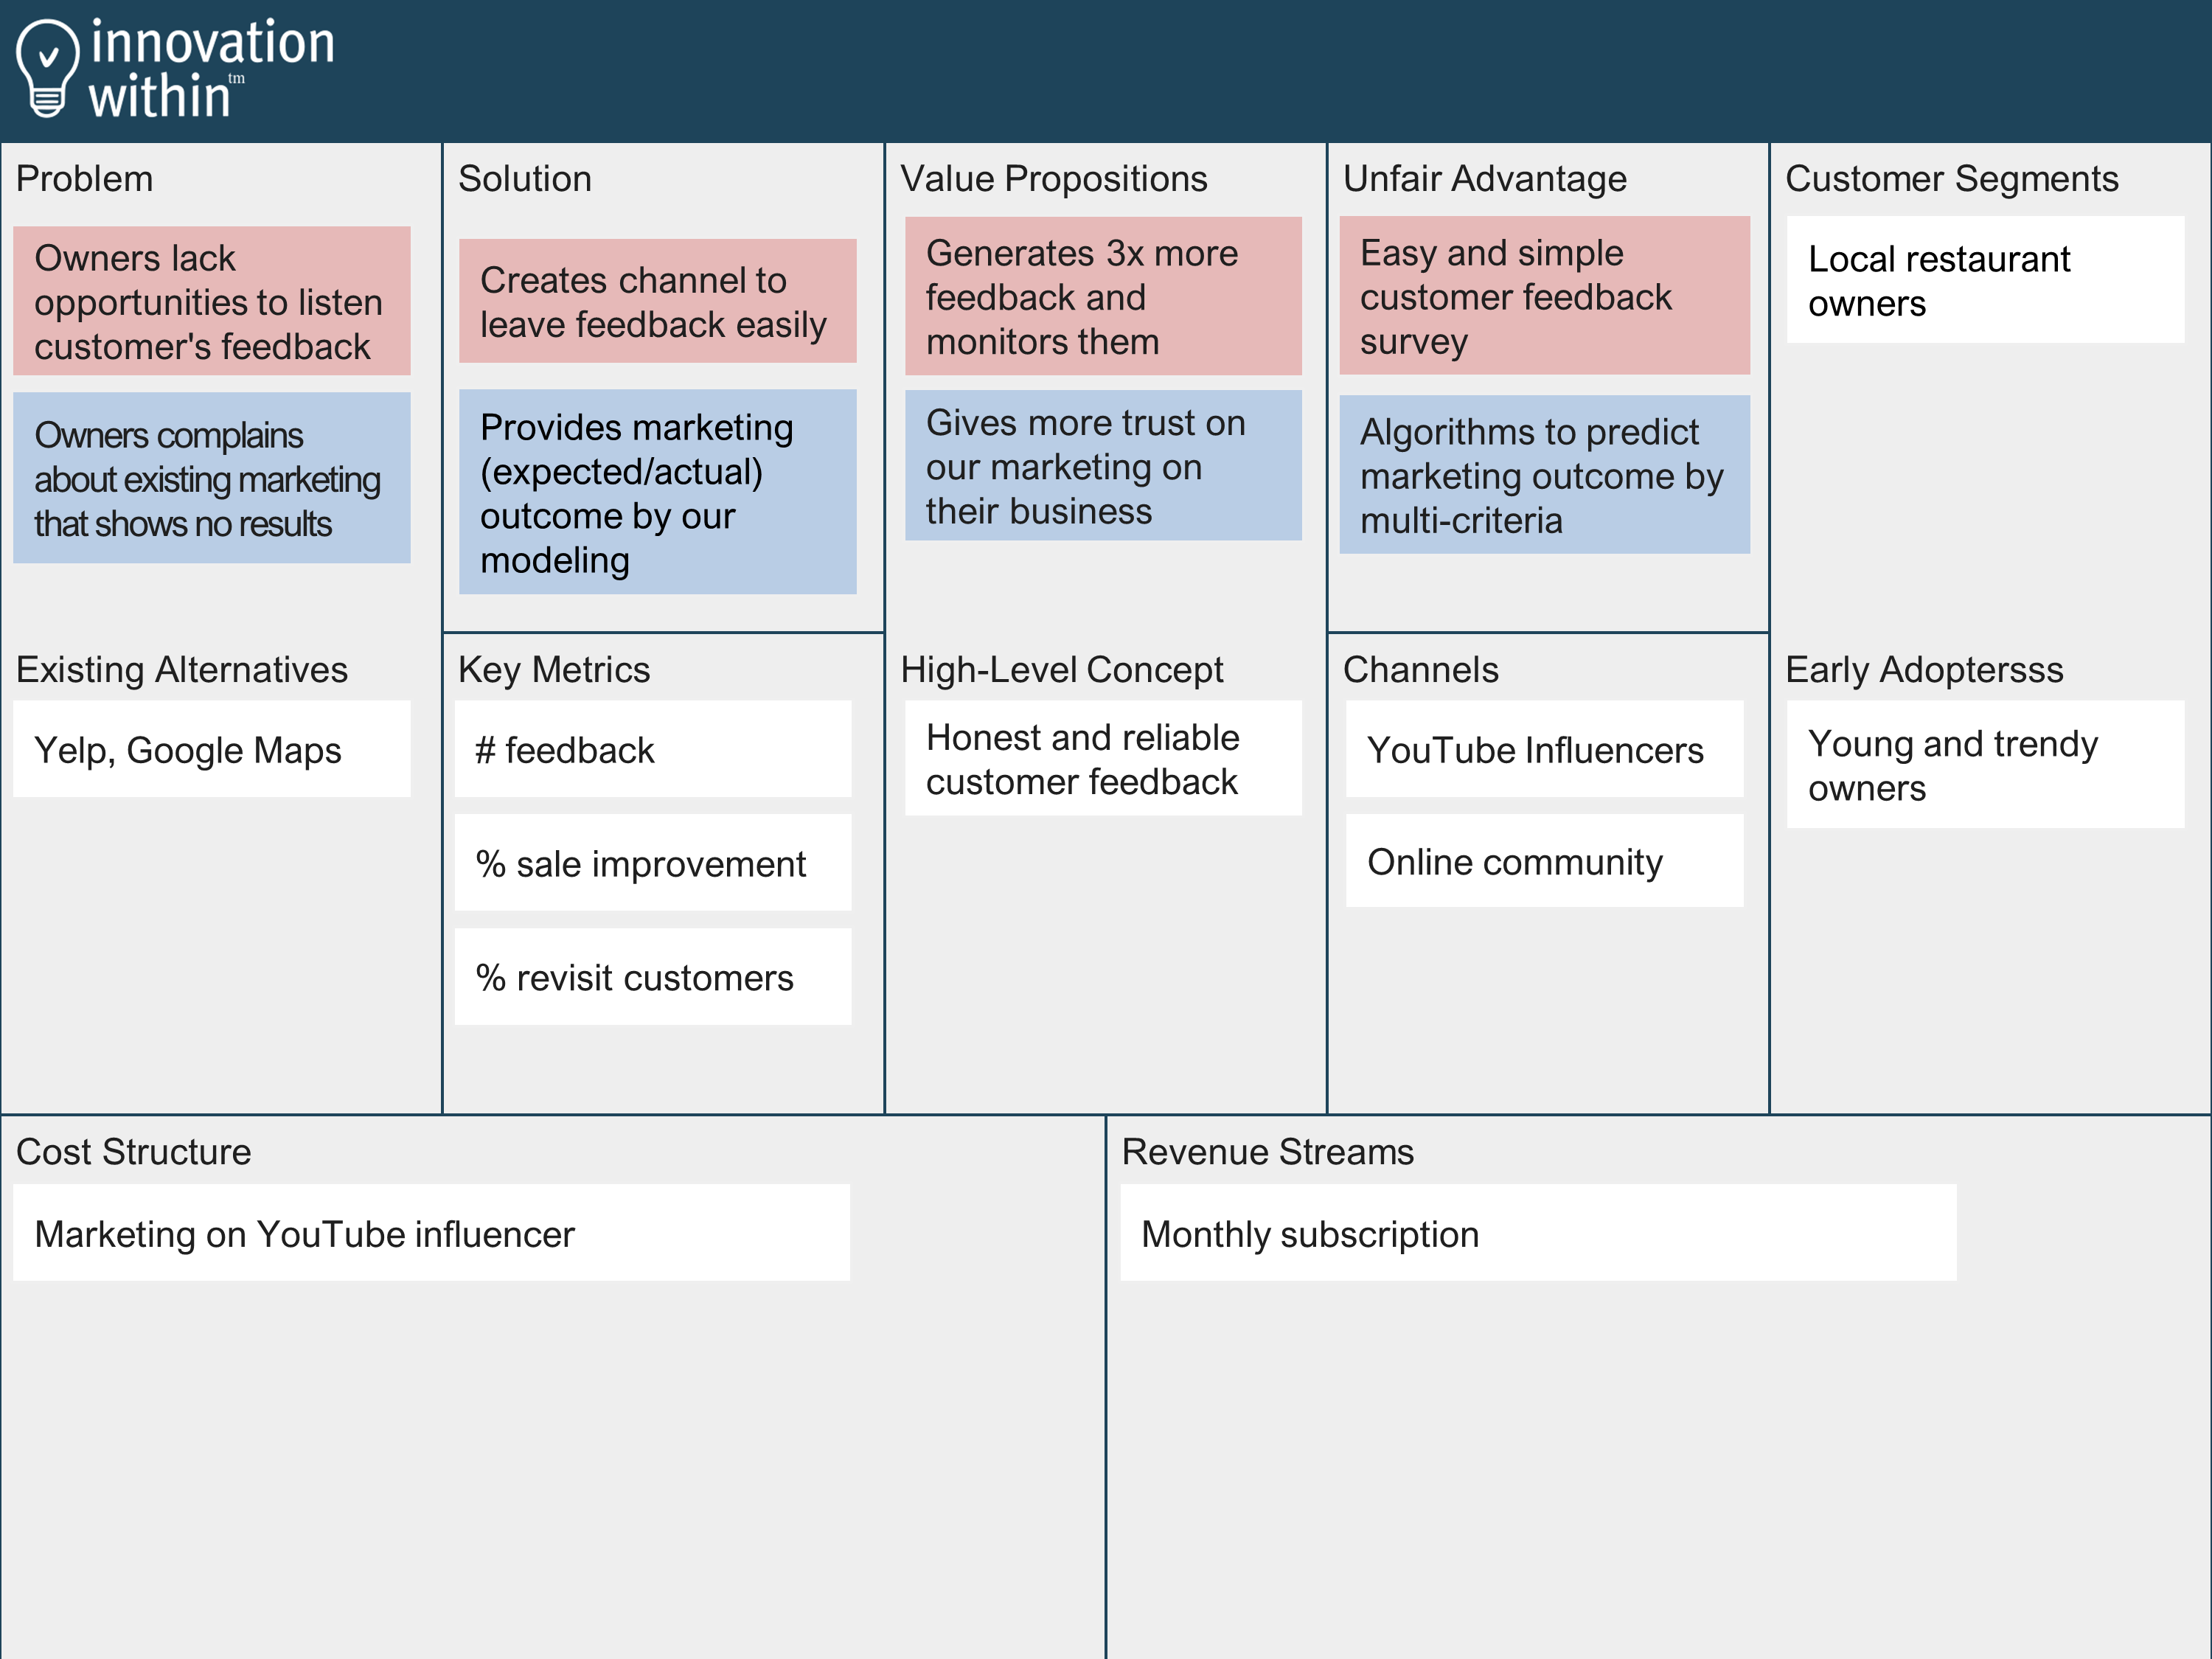
\includegraphics{../image/practical_LL3_3.png}

\hypertarget{uxb370uxbaa8uxb370uxc774}{%
\subsubsection{데모데이}\label{uxb370uxbaa8uxb370uxc774}}

공식적으로 마지막 날인 데모데이는 다른 교육 없이 프로그램을 성공적으로
수행한 것을 축하하는 날이다. 10여개 팀이 선정되어 10분 내외로 프로그램
수행한 것을 발표하고 인스트럭터와 외부 평가의원이 5분간 의견을 준다.
\includegraphics{../image/practical_LL4.png}

\hypertarget{uxd574uxc678-uxc778uxd130uxbdf0-uxd301}{%
\subsubsection{해외 인터뷰
팁}\label{uxd574uxc678-uxc778uxd130uxbdf0-uxd301}}

해외 실전교육은 정량평가 기준인 75개 인터뷰 개수를 채웠는 지가 중요하다.
수월한 인터뷰 수행을 위한 팁은 다음과 같다.

\hypertarget{uxcd9cuxad6d-uxc804-uxc778uxd130uxbdf0uxb97c-uxc7a1uxc544uxb450uxc790}{%
\paragraph{1. 출국 전 인터뷰를
잡아두자}\label{uxcd9cuxad6d-uxc804-uxc778uxd130uxbdf0uxb97c-uxc7a1uxc544uxb450uxc790}}

우리 팀은 미국 출국 전부터 인터뷰를 잡기 위해 노력했다. 영어가
출중하다면 관계 없지만 보다 수월한 인터뷰 수행을 위해, 그리고 미국에
사는 한국인 이야기도 들어봐야 한다고 생각했다.

다른 방법보다도 링크드인으로 동문들에게 연락하는 방법이 가장 유효했다.
UNIST에서 학위를 받은 사람 중 샌프란시스코에서 포스닥을 하거나 직장을
잡으신 분에게 일촌 신청과 메세지를 보냈다. 간략한 내 소개와 메세지를
보내는 이유인 인터뷰 요청, 그리고 간략한 아이템 소개를 담았다.
\includegraphics{../image/practical_interview_linkedin.png} 대부분이
긍정적인 반응과 함께 인터뷰에 응해주셨다. 샌프란시스코 인근 대학인 UCB와
스탠포드에서 연구하는 포스닥 분들을 만날 수 있었고 감사하게도 앞서 말한
시간보다 더 길게 인터뷰를 진행하며 아이템에 대한 고민을 나눌 수 있었다.
\includegraphics{../image/practical_interview_postdoc.png} \#\#\#\# 2.
인터뷰 전략을 세우자 \#\#\#\#\# 일반인 대상 많은 팀이 일반인을 대상으로
고객 탐색 인터뷰를 진행한다. 미국 일반인들도 인터뷰를 구하는 우리의
첫인상을 중요하게 생각할 것이다. 우리는 셔츠나 구두 등 격식을 차리는
복장에 나눠준 명찰을 매고 매 인터뷰에 임했다. 처음 말을 걸 땐, 오늘 하루
어때? 날씨 좋지? 같은 미국식으로 접근하는 방법도 있지만 나의 경우,
정석적으로 명찰을 보여주며, UCB에서 지원하는 창업프로그램에 참여하는
학생인데 고객 탐색 인터뷰를 위해 5분 시간을 내줄 수 있는 지를 묻는 것이
더 반응이 좋았다.
\includegraphics{../image/practical_interview_tip2-1.png}

\hypertarget{uxc18cuxc0c1uxacf5uxc778-uxb300uxc0c1}{%
\subparagraph{소상공인
대상}\label{uxc18cuxc0c1uxacf5uxc778-uxb300uxc0c1}}

우리 팀의 다른 고객은 음식점을 운영하는 소상공인이었다. 무턱대고
미국인이 운영하는 음식점에 찾아가 인터뷰를 구하기 힘들다고 판단한 우리는
한인 음식점을 집중적으로 공략했다. 먼저 샌프란시스코 다운타운과 인근
지역 한식 음식점을 목록화하고 최대한 밥을 그곳에서 사먹고 나오면서
명찰을 드리며 인터뷰를 요청했다. 특히, 한 사장님과 좋은 관계를 유지하면
다른 분들도 소개해주시는 경우도 있었다.
\includegraphics{../image/practical_interview_tip2-2.png}

\hypertarget{uxc124uxbb38uxc870uxc0acuxac00-uxc544uxb2cc-uxb300uxd654uxb97c}{%
\paragraph{3. 설문조사가 아닌
대화를}\label{uxc124uxbb38uxc870uxc0acuxac00-uxc544uxb2cc-uxb300uxd654uxb97c}}

처음 인터뷰는 써놓은 대본을 읽고 예/아니오를 체크하고 넘어가는 경우가
많았다. 상대방 눈을 바라보지 못하고 대화가 아닌 물어보고 답을 적고 하는
것은 인터뷰가 아니라고 한다.
\includegraphics{../image/practical_interview_worst.png} 인터뷰에서
물어볼 내용이 많아도 한 질문에 대해 관심이 있다면 그 근본 원인을 찾기
위해 \href{https://brunch.co.kr/@cliche-cliche/113}{5-Why 기법}으로 다른
질문을 과감히 버리고 집중했다. 녹음 기능을 켜고 최대한 눈을 마주보고
대화를 하려고 했고, 이 경우에 더 많은 시사점을 얻을 수 있었다.
\includegraphics{../image/practical_interview_good.png}



\end{document}
